\documentclass[11pt]{article}
\usepackage{float}
\usepackage{authblk}


%%%%%%%%%% double spacing
\usepackage{setspace}
%\setstretch{2}
%%%%%%%%%%%%%%%%%%%%%%%%%%%%

\usepackage{mathtools}
\usepackage{graphicx}
\usepackage{amssymb}
\usepackage{physics}
\usepackage{hyperref}
\usepackage{comment}
\usepackage{amsmath}
\usepackage{amsthm}
\usepackage{tikz}
\usepackage{bbm}
\usepackage[english]{babel}
\usepackage[autostyle]{csquotes}
\usepackage{forest}
\usetikzlibrary{arrows, arrows.meta, shapes.geometric, calc, shadows, trees}
\usetikzlibrary{decorations.text}


\usepackage{hyperref}
\usepackage{blindtext}
\usepackage{xcolor}
\usepackage{titlesec}
\usepackage[most]{tcolorbox}

%%%%%%%%%%%%%%%%%%%%%%%%%%%%%%%%%%%%%%%%%%%%%%
\newcommand{\ms}[1]{\mathsf{#1}}
%%%%%%%%%%%%%%%%%%%%%%%%%%%%%%%%%%%%%%%%%%%%%%
\tikzstyle{startstop} = [rectangle, rounded corners, 
minimum width=3cm, 
minimum height=1cm,
text centered, 
draw=black, 
fill=red!30]

\tikzstyle{io} = [trapezium, 
trapezium stretches=true, % A later addition
trapezium left angle=70, 
trapezium right angle=110, 
minimum width=3cm, 
minimum height=1cm, text centered, 
draw=black, fill=blue!30]

\tikzstyle{process} = [rectangle, 
minimum width=3cm, 
minimum height=1cm, 
text centered, 
text width=3cm, 
draw=black, 
fill=orange!30]

\tikzstyle{decision} = [diamond, 
minimum width=3cm, 
minimum height=1cm, 
text centered, 
draw=black, 
fill=green!30]
\tikzstyle{arrow} = [thick,->,>=stealth]

%%%%%%%%%%% PAGE COLOR %%%%%%%%%%%%%%%%%%%%%%%%
%\pagecolor[rgb]{0,0,0} %black
%\color[rgb]{1.0,1.0,1.0} %grey
%%%%%%%%%%%%%%%%%%%%%%%%%%%%%%%%%%%%%%%%%%%%%%%
\hypersetup{colorlinks, linkcolor={blue}, citecolor={blue}, urlcolor={blue}}  


%%%%%%%%%%% Sepeartor symbol----***--- %%%%%%%%%%%%%%%%%%%%%%%%%%
\newcommand{\sep}
{
  \begin{center}\begin{tikzpicture}[thick]
  \draw (-1,0) -- (1,0);
  \fill[rotate=45] (-0.075,-0.075) rectangle (0.075,0.075);
  \end{tikzpicture}\end{center}
}

%%%%%%%%%%% PAPER GEOMETRY %%%%%%%%%%%%%%%%%%%%%%%%%%
\usepackage[a4paper, total={6in, 9in}]{geometry}
\DeclarePairedDelimiter\ceil{\lceil}{\rceil}
\DeclarePairedDelimiter\floor{\lfloor}{\rfloor}
\renewcommand*{\Affilfont}{\small\normalfont}

%%%%%%%%%%%%%%%%%%%%%%%%%%%%%%%%%%%%%%%%%%%%%%%%%%%%
%\usepackage{draftwatermark}
%\SetWatermarkText{Accelequant Confidential}
%\SetWatermarkScale{2}

\setcounter{tocdepth}{2}

%%%%%%%%%%%%%%%%%%%%%%%%%%%%%%%%%%%%%%%%%%%%%%%%%%%%
%%%%%%%%%%%%%%%%%% TITLE %%%%%%%%%%%%%%%%%%%%%%%%%%%
%%%%%%%%%%%%%%%%%%%%%%%%%%%%%%%%%%%%%%%%%%%%%%%%%%%%
\usepackage{thmtools,thm-restate}

\newtheorem{theorem}{Theorem}[section]
\newtheorem{definition}{Definition}[section]
\newtheorem{lemma}{Lemma}[section]
\newtheorem{propo}{Proposition}[section]
\newtheorem{coro}{Corollary}[section]
\newtheorem{prob}{Problem}[section]
\newtheorem{hyp}{Hypothesis}[section]
\newtheorem{asmp}{Assumption}[section]
\newtheorem{conj}{Conjecture}[section]
\newtheorem{claim}{Claim}[section]
\newtheorem{fact}{Fact}[section]

%https://tex.stackexchange.com/questions/422/how-do-i-repeat-a-theorem-number
\begin{comment}
    \makeatletter
\newtheorem*{rep@theorem}{\rep@title}
\newcommand{\newreptheorem}[2]{%
\newenvironment{rep#1}[1]{%
 \def\rep@title{#2 \ref{##1}}%
 \begin{rep@theorem}}%
 {\end{rep@theorem}}}
\makeatother
\end{comment}

\newtheorem{subdefinition}{Definition}[definition]
\renewcommand{\thesubdefinition}{\thedefinition\alph{subdefinition}}

\newtheorem{innercustomthm}{Theorem}
\newenvironment{customthm}[1]
  {\renewcommand\theinnercustomthm{#1}\innercustomthm}
  {\endinnercustomthm}

\newtheorem{innercustomdef}{Definition}
\newenvironment{customdef}[1]
  {\renewcommand\theinnercustomdef{#1}\innercustomdef}
  {\endinnercustomdef}

\newtheorem{innercustomcor}{Corollary}
\newenvironment{customcor}[1]
  {\renewcommand\theinnercustomcor{#1}\innercustomcor}
  {\endinnercustomcor}

\newtheorem{innercustomconj}{Conjecture}
\newenvironment{customconj}[1]
  {\renewcommand\theinnercustomconj{#1}\innercustomconj}
  {\endinnercustomconj}



\theoremstyle{definition}
\newtheorem{example}{Example}[section]
\newtheorem{remark}{Remark}[section]

\newcommand{\jordi}[1]{{\bf\color{red}Jordi: [#1]}}
\newcommand{\marten}[1]{{\bf\color{blue}Marten: [#1]}}
\newcommand{\chris}[1]{{\bf\color{orange}Chris: [#1]}}
\newcommand{\com}[1]{{\bf\color{purple}Comment: [#1]}}
\newcommand{\newtxt}[1]{{\bf\color{purple}New text: [#1]}}


%%%%%%%%%%%%%%%%%%%%%%%%%%%%%%%%%%%%%%%%%%%%%%%%%%%%%%%%%%%%
%%%%%%%%%%%%%%% Bra-Ket notation %%%%%%%%%%%%%%%%%%%%%%%%%%%
\newcommand{\si}{\ket{\psi}}
\newcommand{\fii}{\ket{\phi}}
\newcommand{\zii}{\ket{\textbf{z}}}


%%%%%%%%%%%%%%%%%%%%%%%%%%%%%%%%%%%%%%%%%%%%%%%%%%%%%%%%%%%%%%%%
%%%%%%%%%%%%%%%% BF MATH %%%%%%%%%%%%%%%%%%%%
\newcommand{\xx}{\mathbf{x}}
\newcommand{\yy}{\mathbf{y}}
\newcommand{\zz}{\mathbf{z}}
\newcommand{\vv}{\mathbf{v}}
\newcommand{\uu}{\mathbf{u}}
\newcommand{\mm}{\mathbf{m}}
\newcommand{\kk}{\mathbf{k}}
\newcommand{\cc}{\mathbf{c}}
\renewcommand{\S}{\mathbf{S}}
\newcommand{\bb}{\mathbf{b}}


%%%%%%%%%%%%%%%%%%%%%%%%%%%%%%%%%%%%%%%%%%%%%%%%%%%%%%%%%%%%%%%%
%%%%%%%%%%%%%%%%%%%%%%% MATH-CAL %%%%%%%%%%%%%%%%%%%%%%%%%%%%%%%%
\newcommand{\mA}{\mathcal{A}} 
\newcommand{\mC}{\mathcal{C}} 
\newcommand{\mH}{\mathcal{H}}
\newcommand{\mO}{\mathcal{O}}
\newcommand{\mW}{\mathcal{W}}
\newcommand{\mN}{\mathcal{N}}
\newcommand{\mS}{\mathcal{S}}
\newcommand{\cS}{\mS}
\newcommand{\LL}{\mathcal{L}}
\newcommand{\OO}{\mathcal{O}}
\renewcommand{\AA}{\mathcal{A}}
\newcommand{\MM}{\mathcal{M}}
\newcommand{\HH}{\mathcal{H}}


%%%%%%%%%%%%%%%%%%%%%%%%%%%%%%%%%%%%%%%%%%%%%%%%%%%%%%%%%%%%%%%%
%%%%%%%%%%%%%%%%%%%%%%%% MATHBB %%%%%%%%%%%%%%%%%%%%%%%%%%%%%%%%
%%%%%%%%%%%%%%%%%%%%%%%%%%%%%%% BB MATH %%%%%%%%%%%%%%%%%%%%%%%%%%%%%%%%%%%%
\newcommand{\N}{\mathbb{N}}
\newcommand{\C}{\mathbb{C}}
\newcommand{\Z}{\mathbb{Z}}
\newcommand{\Q}{\mathbb{Q}}
\newcommand{\R}{\mathbb{R}}


%%%%%%%%%%%%%%%%%%%%%%%%%%%%%%%%%%%%%%%%%%%%%%%%%%%%%%%%%%%%%%%%
%%%%%%%%%%%%%%%%%%%%%%% MATH-SF %%%%%%%%%%%%%%%%%%%%%%%%%%%%%%%%
%%%%%%%%%%%%%%% COMPLEXITY CLASSES %%%%%%%%%%%%%%%%%%%%%%%
\renewcommand{\P}{\mathsf{P}}
\newcommand{\NC}{\mathsf{NC}}
\newcommand{\QNC}{\mathsf{QNC}}
\newcommand{\BQNC}{\mathsf{BQNC}}
\newcommand{\Pclass}{\mathsf{P}}
\newcommand{\RP}{\mathsf{RP}}
\newcommand{\BPP}{\mathsf{BPP}}
\newcommand{\BQP}{\mathsf{BQP}}
\newcommand{\NP}{\mathsf{NP}}
\newcommand{\NqP}{\mathsf{NqP}}
\newcommand{\MA}{\mathsf{MA}}
\newcommand{\AM}{\mathsf{AM}}
\newcommand{\UMA}{\mathsf{UMA}}
\newcommand{\QMA}{\mathsf{QMA}}
\newcommand{\bQMA}{\mathsf{$\beta$QMA}}
\newcommand{\UQMA}{\mathsf{UQMA}}
\newcommand{\QCMA}{\mathsf{QCMA}}
\newcommand{\bQCMA}{\mathsf{$\beta$QCMA}}
\newcommand{\UQCMA}{\mathsf{UQCMA}}
\newcommand{\PCP}{\mathsf{PCP}}
\newcommand{\PSPACE}{\mathsf{PSPACE}}
\newcommand{\QPCP}{\mathsf{QPCP}}
\newcommand{\QCPCP}{\mathsf{QCPCP}}
\newcommand{\SPCP}{\mathsf{SPCP}}
\newcommand{\PH}{\mathsf{PH}}
\renewcommand{\BQP}{\mathsf{BQP}}
\newcommand{\PBQP}{\mathsf{PreciseBQP}}
\newcommand{\StoqMA}{\mathsf{StoqMA}}

%%%%%%%%%%%%%%%%%%%%%%%% TURING MACHINE %%%%%%%%%%%%%%%%%%%%%%%%%%%%%
\newcommand{\TM}{\mathsf{TM}}
\newcommand{\QTM}{\mathsf{QTM}}
\newcommand{\NTM}{\mathsf{NTM}}
\newcommand{\QNTM}{\mathsf{QNTM}}

%%%%%%%%%%%%%%% LOCAL HAMILTONIAN %%%%%%%%%%%%%%%%%%%%%%%
\newcommand{\LH}{\mathsf{LH}}
\newcommand{\FH}{\mathsf{FH}}
\newcommand{\SAT}{\mathsf{SAT}}
\newcommand{\QFT}{\mathsf{QFT}}
\newcommand{\QPE}{\mathsf{QPE}}
\newcommand{\LHES}{\mathsf{LHES}}
\newcommand{\hist}{\mathsf{hist}}
\newcommand{\CC}{\mathsf{C}}
\newcommand{\ILP}{\mathsf{ILP}}
\newcommand{\GuLH}{\text{GuLH}}
\newcommand{\UQA}{\mathsf{UQA}}
\newcommand{\GLH}{\mathsf{GLH}}
\newcommand{\GLHgd}{\mathsf{GLH(k, $\gamma$, $\delta$)}}
\newcommand{\GaLH}{\mathsf{GaLH}}
\newcommand{\GaLHgd}{\mathsf{GaLH(k, $\gamma$, $\delta$)}}
%%%%%%%%%%%%%%% Promise PROBLEM %%%%%%%%%%%%%%%%%%%%%%%
\newcommand{\Yes}{\mathsf{Yes}}
\newcommand{\No}{\mathsf{No}}
\newcommand{\Input}{\mathsf{Input}}
\newcommand{\Output}{\mathsf{Output}}
\newcommand{\Promise}{\mathsf{Promise}}
\newcommand{\Goal}{\mathsf{Goal}}
\newcommand{\Proof}{\mathsf{Proof}}
%%%%%%%%%%%% Functions %%%%%%%%%%%%%%%%%%%%%%%%%%%%
\renewcommand{\exp}{\mathsf{exp}}
\renewcommand{\log}{\mathsf{log}}
\newcommand{\poly}{\mathsf{poly}}
\newcommand{\polylog}{\mathsf{polylog}}
\newcommand{\logpn}{\mathsf{O(log^p n)} }

%%%%%%%%%%%%%%%%%%%%%%%%%%%%%%%%%%%%%%%%%%%%%%%%%%
%%%%%%%%%%%%%%% MATH FRACK %%%%%%%%%%%%%%%%%%%%%%%
\newcommand{\fn}{\mathfrak{n}}
\newcommand{\fC}{\mathfrak{C}}
\newcommand{\expp}{\mathop{exp}}


%\renewcommand{\Pr}{\textrm{Pr}}
\renewcommand{\Tr}{\textrm{Tr}}

\newcommand{\kb}[2]{|#1\rangle\langle#2|}
\newcommand{\proj}[1]{|#1\rangle\langle#1|}
\newcommand{\ot}{\otimes}

\newcommand{\hatt}[1][]{\hat{t#1}}


\title{Spectral Characterization of $\mathsf{QMA}$  }
%%%%%%%%%%%%%%%%%%%%%%%%%%%%%%%%%%%%%%%%%%%%%%%%%%%%%%
%%%%%%%%%%%%%%%%%%%%%%%%% AUTHORS %%%%%%%%%%%%%%%%%%%%
%%%%%%%%%%%%%%%%%%%%%%%%%%%%%%%%%%%%%%%%%%%%%%%%%%%%%%
%\author{Manish Kumar\footnote{manish@accelequant.com} \\ Krishna V. Palem\footnote{krishna@accelequant.com} \\ (Accelequant India Pvt. Ltd.)}

\author[1]{Manish Kumar \footnote{\textcolor{blue}{manish@accelequant.com}\\ \textcolor{red}{Accelequant confidential. Do not copy and distribute.}}}

\author[1]{Krishna V. Palem}

\affil[1]{Accelequant Inc.}

%%%%%%%%%%%%%%%%%%%%%% WATERMARK %%%%%%%%%%%%%
\usepackage{background}
\backgroundsetup{
  position=current page.east,
  angle=-90,
  nodeanchor=east,
  vshift=-5mm,
  opacity=1,
  scale=3,
  contents= %Accelequant confidential
}
%%%%%%%%%%%%%%%%%%%%%%%%%%%%%%%%%%%%%%%%%%%%%%

\begin{document}

\maketitle
\begin{abstract}
    We explore the intermediate region between $\mathsf{BQP}$ and $\mathsf{QMA}$-$\mathsf{complete}$ sets using the concept of limited quantum non-determinism and propose an infinite hierarchy of quantum complexity classes between them. Each level in the hierarchy is defined by the size of the quantum circuit required to decide a problem at that level. We also provide an equivalent definition of the hierarchy in the quantum Turing model. Furthermore, we prove that the hierarchy is robust in a certain relativized setting.\par
    Additionally, we propose a complete (promise) problem for each level in the infinite hierarchy named parametrized $\mathsf{Guided}$ $\mathsf{Local}$ $\mathsf{Hamiltonian}$ ($\ms{GLH_i}$). Subsequently, we define and quantify a Fourier spectral concentration of the $\ms{GLH_i}$ problem. Ultimately, this value is used to design a quantum algorithm that harnesses it. To design the quantum algorithm, we repurpose the quantum phase estimation algorithm and incorporate suitable classical pre- and post-processing techniques. As expected, the algorithm's execution time worsens as the spectral concentration of a given problem decreases.\par
\end{abstract}
\newpage

%%%%%%%%%%%%%%%%%%%%%%%%%%%%%%%%%%%%%%%%%%%%%%%%%%%%%%%%%%%%%%%%
\tableofcontents

\newpage
%%%%%%%%%%%%%%%%%%%%%%%%%%%%%%%%%%%%%%%%%%%%%%%%%%%%%%%%%%%%%%%%%
%%%%%%%%%%%%%%%%%%%%%%%%%%%%%%%%%%%%%%%%%%%%%%%%%%%%%%%%%%%%%%%%%
%%%%%%%%%%%%%%%%%%% INTRODUCTION %%%%%%%%%%%%%%%%%%%%%%%%%%%%%%%%
%%%%%%%%%%%%%%%%%%%%%%%%%%%%%%%%%%%%%%%%%%%%%%%%%%%%%%%%%%%%%%%%%
%%%%%%%%%%%%%%%%%%%%%%%%%%%%%%%%%%%%%%%%%%%%%%%%%%%%%%%%%%%%%%%%%

\begin{comment}
    \section{Introduction}
The quantum complexity class $\mathsf{QMA}$ contains several interesting natural problems due to the containment of the sets $\mathsf{P}$, $\NP$, and $\mathsf{BQP}$ in it. Some of the types of practical problems are (i) the classical constraint satisfaction problem ($\mathsf{CSP}$), (ii) low-temperature many-body physics\footnote{To be precise, the decision problem on determining the minimum eigenvalue of such a system.}, and (iii) simulation of quantum and classical systems.\par

Until now, problems in $\mathsf{QMA}$ have been studied in dichotomic settings, which resonate well with the understanding that the problems in $\mathsf{BQP}$ are easy and $\mathsf{QMA}$-complete problems are intractable\footnote{Throughout the paper, we assume the conjecture $\mathsf{P \neq BQP\neq QMA}$ holds.}. Cubitt \& Montanaro studied the quantum analog of Schaefer's dichotomy, a criterion that classifies a $\mathsf{CSP}$ instance either in $\mathsf{P}$ or $\NP$-complete set. They analyzed the quantum analogue of $\mathsf{CSP}$ called the $k$-local Hamiltonian ($k$-$\LH$) problem and classified any $k$-$\LH$ instances into (i) $\mathsf{P}$, (ii) $\NP$, (iii) $\mathsf{stoqMA}$, and (iv) $\mathsf{QMA}$-complete sets based on certain syntactic characterizations of the terms of local Hamiltonian matrices \cite{cubitt2016complexity}. This is a coarse-grained classification of the local Hamiltonian problem. To our knowledge, few studies have examined the fine-grained classification of the $k$-$\LH$ problem. To be more precise, classification into an infinite hierarchy of classes between $\mathsf{BQP}$ and $\mathsf{QMA}$-complete sets. \par

In this article, we initiate the study of a fine-grained complexity classification of problems between $\mathsf{BQP}$ and $\mathsf{QMA}$-complete sets, using the notion of limited quantum nondeterminism. This can be intuitively understood as a quantum nondeterministic Turing machine allowed to make a limited number of quantum nondeterministic steps. The classical counterpart of this limited nondeterminism was studied by Kintala \& Fisher \cite{Kintala1980-yv}. They conjectured non-determinism adds non-trivial power to the computation.\footnote{This is a conjecture as it is still unknown if $\P \neq \NP$. Creating a robust hierarchy between P and $\NP$ only makes sense if the conjecture holds.} Alternatively, if a Turing machine is increasingly allowed to make more nondeterministic steps, it can strictly compute more new problems than before. We have extended and formalized this idea for quantum nondeterminism in this article within the circuit model of quantum computation \cite{yao1993quantum}. With these thoughts in mind, the first guiding question of this work is: Are there some natural problems that can be computed using the limited amount of quantum nondeterminism?\par

To proceed in this direction, we place a new problem in the hierarchy. This has been accomplished by carefully modifying and generalizing the existing $\mathsf{QMA}$ to include problems such as the $\mathsf{LH}$ problems. We also provide an end-to-end quantum algorithm for computing these problems by (i) providing a method to generate an ansatz state and (ii) employing the quantum phase estimation algorithm to determine the ground energy. The running time of the algorithm depends on the amount of non-deterministic guessing required to solve the problem. As expected, the asymptotic running time is superpolynomial, and it worsens significantly for problems higher in the hierarchy.\par

%%%%%%%%%%%%%%%%%%%%%%%%%%%%%%%%%%%%%%%%%%%%%%%%%%%%%%%%%%%%%%%%
%%%%%%%%%%%%%%%%%%%%%%%%%%%%%%%%%%%%%%%%%%%%%%%%%%%%%%%%%%%%%%%%
%%%%%%%%%%%%%%%%%%%%%%%%%%%%% INTRODUCTION %%%%%%%%%%%%%%%%%%%%%%
%%%%%%%%%%%%%%%%%%%%%%%%%%%%%%%%%%%%%%%%%%%%%%%%%%%%%%%%%%%%%%%%
%%%%%%%%%%%%%%%%%%%%%%%%%%%%%%%%%%%%%%%%%%%%%%%%%%%%%%%%%%%%%%%%
\newpage
\end{comment}

\section{The Internal Structure of $\ms{QMA}$}
We characterize the complexity of natural problems in $\ms{QMA}$ through a hierarchy starting from $\ms{BQP}$ and extending to problems complete for $\ms{QMA}$. We start with a quantum circuit-based definition of our hierarchy, building on the concept of promise problems. We will now review some basic definitions.

\subsection{Preliminary definitions}
We will mostly deal with a promise problem, which is a generalization of the notion of a language.
\begin{definition}
    [Promise problem] A promise problem $\mathcal{A} \equiv \{\mathcal{A}_{yes}, \mathcal{A}_{no}\}$ where $\mathcal{A}_{yes}$ and $\mathcal{A}_{no}$ are a set of accepted and a set of rejected inputs, respectively. Additionally, the sets $\mathcal{A}_{yes},\mathcal{A}_{no}\subseteq \{0,1\}^*$. A set of invalid inputs are defined as $ \mathcal{A}_{inv}\equiv \{0,1\}^*\backslash{} \{\mathcal{A}_{yes}\cup \mathcal{A}_{no}\}$ which may not be an empty set. A promise problem becomes a language as a special case when $\mathcal{A}_{inv}$ is the empty set.
\end{definition}
It should be noted that an algorithm deciding a promise problem is usually not provided with an input in $x\in \mathcal{A}_{inv}$. Nevertheless, if invalid inputs are provided to the algorithm, it may accept or reject them arbitrarily.
\par Since a quantum circuit of fixed size can only take an input of fixed size, a promise problem is decided by a family of circuits that consists of a set of circuits $\{Q_n\}_{n\in \N}$, each for a different input size. It is formally defined as follows.
\begin{definition}
    [$U(n)$-uniform quantum circuit family] Let $U(n): \N \rightarrow \N$ be a function. A family of quantum circuits $\{Q_n\}_{n\in \N}$ is called $U(n)$-uniform if there exists a classical Turing machine that takes $1^{n}$ as input and outputs a classical description of the quantum circuit $Q_n$ of size $O(U(n))$ in time at most $\poly(U(n))$.
\end{definition}
When the function $U(n)$ is some polynomial, this special case is called a $P$-uniform quantum circuit. Building upon these definitions, we review the quantum circuit-based definition of a set of promise problems decided by a uniformly generated quantum circuit of a certain size.
\begin{definition}
    [$\ms{BQSIZE}(s(n))$] A promise problem $\mathcal{A} \equiv \{\mathcal{A}_{yes}, \mathcal{A}_{no}\}$ is in $\ms{BQSIZE}(s(n))$ if and only if there exists a $\poly(s(n))$-uniform family of quantum circuits $\{Q_n\}_{n\in \N}$ such that if $x\in \mathcal{A}_{yes}$, then   
    $${Pr[Q_n\ \textrm{accepts}\ x]\geq 2/3},$$
    
    while, if $x\not\in \mathcal{A}_{no}$, then 
    $${Pr[M\ \textrm{accepts}\ x]\leq 1/3}.$$
    
    $\ms{BQSIZE}[s(n)]$ is defined as the class of all promise problems decided by quantum circuits of size ${O(s(n))}$.
\end{definition}
This definition is an adapted version of a definition for $\ms{BQTIME}(T(n))$ given in terms of a quantum Turing machine by in \cite{fortnow2004promise}. We argue its equivalence in section \ref{sec: turing vs circuit}.\par
Another important class of interest is $\ms{QMA}$ whose circuit-based definition is as follows.

\begin{definition}
    [$\mathsf{QMA}$ complexity class] A promise problem $\mathcal{A}$ is in $\mathsf{QMA}$ if and only if there exists a P-uniform quantum circuit family $\{Q_n\}_{n\in \N}$ and a polynomial $p:\N \rightarrow \N$, such that the circuit $Q_n$ takes as input a string $\xx\in \mathcal{A}$ and decides on acceptance or rejection of $\xx$ as below.
    \begin{itemize}
        \item If $\xx\in \mathcal{A}_{yes} \implies$ $\exists\si\in (\C^2)^{\otimes p(|\xx|)}$, ${Pr[Q\ accepts\ \{\xx,\ket{\psi}\}]}$ $\geq 2/3$.
        \item If $\xx\in \mathcal{A}_{no} \implies $ $\forall \si\in (\C^2)^{\otimes p(|\xx|)}$, ${Pr[Q\ accepts \{\xx,\ket{\psi}\} ]}$ $\leq 1/3$.
    \end{itemize}
\end{definition}

\subsection{$\ms{QMAH}$: An infinite hierarchy in $\ms{QMA}$ }
We define individual levels in the $\ms{QMAH}$ hierarchy as follows.
\begin{definition}
    [$\ms{QMAH}_f$] For a specified function $f:\N \rightarrow\N$, a promise problem $\mathcal{A} $ is in $\ms{QMAH}_f$, a level of $\ms{QMAH}$, if and only if it belongs to $\QMA$ as well as $\ms{BQSIZE}[f(n)]$.
    \label{def: QMAH_f}
\end{definition}
Later on, we conditionally prove that if for any two functions $f_1$ and $f_2$, where $f_2$ asymptotically grows faster than $f_1$, then $\ms{QMAH}_{f_1}$ is strictly contained in $\ms{QMAH}_{f_2}$. Alternatively, $f_1\in o(f_2)$ implies $\ms{QMAH}_{f_1}\subset \ms{QMAH}_{f_2}$ under the standard assumption of $\BQP \neq \QMA$. \par
To emphasize the role of choosing two functions, we employ the notion of a parametrized family of functions whose members have an asymptotic growth rate that is faster than any polynomial but slower than any exponential function. The latter restriction on growth with respect to an exponential function is motivated by the fact that $\ms{QMA}$ is contained in $\mathsf{EXP}$, the set of problems that can be solved by a Turing machine in exponential time. Thus, $f_1$ and $f_2$ growing faster than any exponential function would trivially imply $\ms{QMAH}_{f_1}=\ms{QMAH}_{f_2}$ because any problem in $\ms{QMA}$ can be decided in $O(2^n)$ time using a classical Turing machine. Similarly, we want the growth of $f_1$ and $f_2$ to be asymptotically faster than any polynomial. Otherwise, the problem is trivially in $\ms{BQP}$. Thus, the intermediate growth rate of $f_1$ and $f_2$ enable us to establish $\ms{QMAH}_{f_1}\subset \ms{QMAH}_{f_2}$ under a plausible assumption of $\ms{BQP\neq QMA}$.

\begin{definition}
    [Indexed family of functions] We define an indexed family of functions as a set of functions whose elements are functions indexed by integers. Formally, $F:=\{f_i\ |\ \forall i,j\in \N, f_i\in o(f_j)\ \textrm{if}\ i<j. \}$
\end{definition}
We define our hierarchy as follows.
\begin{definition}
    [$\ms{QMAH_i}$: Level-$i$ of the hierarchy] For any specified positive integer $i\in \mathbb{N}$, a promise problem $\mathcal{A}$ is in $\ms{QMAH_i}$, the $i^{th}$ level of $\ms{QMAH}$, if and only if it belongs to $\QMA$ as well as $\ms{BQSIZE}[f_i]$.
    \label{def: QMAH_i}
\end{definition}

There are numerous examples of the parametrized family of functions. For the sake of brevity, we illustrate it with the indexed family of quasi-polynomial functions given by $F\equiv \{f_i:=2^{O(\log^i (n))}\ |\ i\in \N \}$. This naturally instantiate our hierarchy as follows.\footnote{it should be noted that for $i=1$, $f_1=2^{O(\log(n))}=\bigcup_{c\in \N }2^{c\cdot\log(n)} = \bigcup_{c\in \N }2^{\log(n^c)}$. It can be demonstrated that any polynomial function $g(x)=n^d$ is an element of $f_1$. In fact, $f_1$ is exactly the set of all polynomial functions. Or, every element of $f_1$ is a polynomial of some degree.}

\begin{comment}
    =\bigcup_{c\in \N }2^{\log(n^c)}=\bigcup_{c\in \N }{n^c}
\end{comment}

\begin{definition}
    [$\ms{QMAH_i}$: Level-$i$ of the hierarchy] For any specified positive integer $i\in \mathbb{N}$, a promise problem $\mathcal{A}$ is in $\ms{QMAH_i}$, the $i^{th}$ level of $\ms{QMAH}$, if and only if it belongs to $\QMA$ as well as $\ms{BQSIZE}[2^{O(\log^i(n))}]$.
    \label{def: QMAH_i}
\end{definition}

In this setting, the associated $\ms{QMAH}$ hierarchy is defined to be a union of the classes $\mathsf{QMAH_i}$ for all positive integers $i\in \mathbb{N}$.
\begin{definition}
    [$\ms{QMAH}$ Hierarchy] $\ms{QMAH}$ is defined as an infinite union of $\ms{QMAH_i}$ for all positive integer $i\in \mathbb{N}$. $$\ms{QMAH\equiv\bigcup_{i\in \mathbb{N}}QMAH_i}.$$
\end{definition}
Now we determine the position of the hierarchy with respect to the complexity classes $\ms{QMA}$, and $\ms{BQP}$.
\begin{theorem}
    The hierarchy $\ms{QMAH \subseteq QMA}.$
\end{theorem}
\textbf{Proof:} Definition of each level of the hierarchy dictates  $\ms{QMAH_i \subseteq QMA}$ for $\forall i\in \N$. To proof $$\ms{QMAH\equiv \bigcup_{i\in \mathbb{N}} QMAH_i \subseteq QMA},$$ we provide the following set-theoretic argument. Take any $x\in \bigcup_{i\in \mathbb{N}} \ms{QMAH}_i$. Then, there must be an $i\in \N$ such that $x\in \ms{QMAH}_i$. Since $\ms{QMAH_i}\subseteq \ms{QMA}$ for all $i\in \N$, thus $x\in \ms{QMA}$ too.      \qed

\begin{theorem}
    The first level of the hierarchy $\ms{QMAH_1 = BQP}.$
\end{theorem}
\textbf{Proof:} The proof of $\ms{BQP\subseteq QMAH_1}$ is due to the fact that $\ms{BQP}$ is in (i) $\ms{QMA}$ and (ii) $\bigcup_{c\in \mathbb{N}} \ms{BQSIZE(n^c) = BQSIZE(2^{O(log\ n)}})$. For the other direction, $\ms{QMAH_1\subseteq BQP}$, we use the fact that the set of promise problems in $\ms{QMA}$ with a polynomial time algorithm is the same as $\ms{BQP}$. \qed

\begin{figure}[ht]
    \centering
    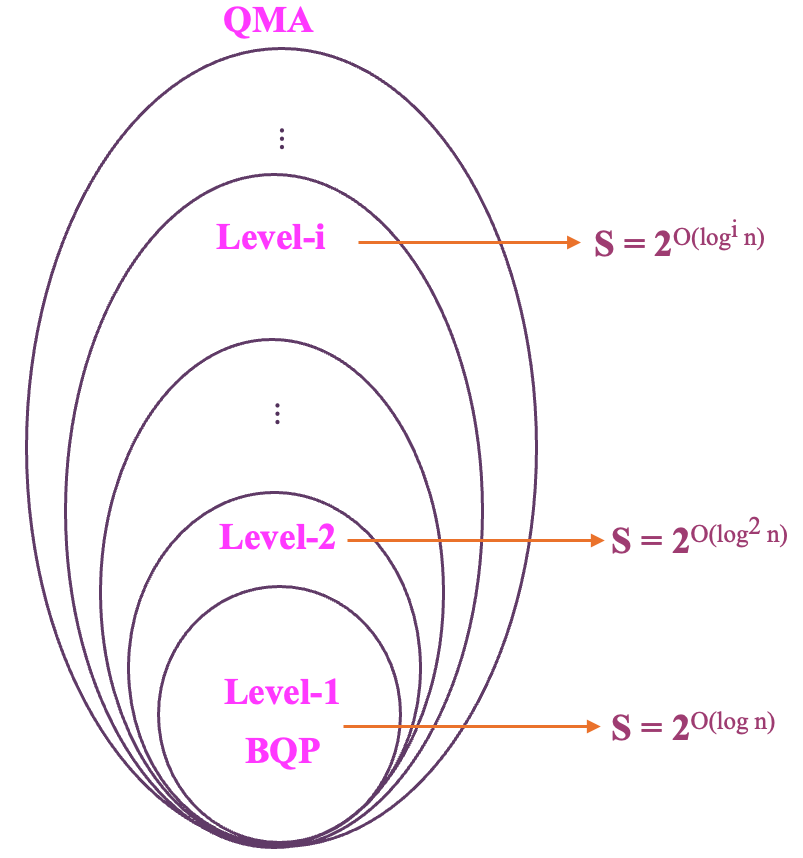
\includegraphics[width=0.50\textwidth]{pics/Hierarchy_Sizewise.png}
    \caption{ We define an infinite hierarchy in $\ms{QMA}$. In one of the instantiations of the hierarchy, the level-$i$ in the hierarchy is a set of promise problems in $\ms{QMA}$ for which there is a quantum Turing machine that decides the problem using at most $\ms{2^{O(log^i n)}}$ steps. As argued in the main text, the choice of the indexed family of functions as $F\equiv \{2^{O(\log^i (n))}|i\in \N\}$ is solely for an illustrative reason. One can choose another indexed family of functions as long as they fulfill two properties characterizing the asymptotic growth of the constituent functions.}
    \label{fig:level-hierarchy}
\end{figure}
%%%%%%%%%%%%%%%%%%%%%%%%%%%%%%%%%%%%%%%%%%%%%%%%%%%%%%%%%%%%%%%%%%%%%%%%%%%

%%%%%%%%%%%%%%%%%%%%%%%%%%%%%%%%%%%%%%%%%%%%%%%%%%%%%%%%%%%%%%%%%%%%%%%%%%%
\subsection{Defining $\mathsf{QMAH}$ through Quantum Turing machine}\label{sec: turing vs circuit}
The definition of the hierarchy in the previous section strictly adheres to the quantum circuit model of quantum computation. In this section, we provide an alternative yet equivalent definition of the hierarchy in the quantum Turing model, which is arguably less prevalent than other models of quantum computing. We start with reviewing the equivalence of these two models proven by \cite{yao1993quantum}, and then present the definition of $\mathsf{QAMH}$ in terms of the Quantum Turing model of computation.
\subsubsection{Known equivalence between Turing and Circuit model of quantum computation}
For the sake of completeness, we review the key differences between the quantum Turing and the quantum circuit models, followed by a discussion of the precise technical sense in which the models are equivalent.
\begin{definition}
    [\cite{vazirani2002survey}]A quantum Turing machine ($\mathsf{QTM}$) is defined by a triplet $(\Sigma, S,\delta)$, where $\Sigma$ is a finite alphabet with an identified blank symbol $\#$, $S$ is a finite set of states with an identified initial state $s_0$ and final state $s_f$, and $\delta$, the quantum finite state control is a function 
    \begin{equation}
        \delta: S\times \Sigma \mapsto \mathbb{C}^{\Sigma\times S\times D}
    \end{equation}
    with $D=\{L,R\}$. The quantum Turing machine has a two-way infinite tape of cells indexed by the integers $\mathbb{Z}$ and a single read/write tape that steps along it.
\end{definition}
A quantum circuit is a generalization of a classical reversible circuit with the following three fundamental changes.
\begin{enumerate}
    \item Classical registers are replaced by quantum registers.
    \item A classical reversible gate set (say, $\{\ms{Toffoli}\}$) is replaced with a universal quantum gate set, say $\{ \ms{Toffoli},\ \ms{Hadamard}\}$.
    \item Quantum measurement in a specified basis (say, standard basis) is deployed at the end of the computation to read out the output.
\end{enumerate}

%\subsubsection{Equivalence between a Turing and a circuit model of computation}
The equivalence between the quantum Turing model and the quantum circuit model of computation was established by Andrew Yao \cite{yao1993quantum}. We summarize their equivalence by specifying the precise notion of a quantum circuit that simulates a quantum Turing machine.
\begin{comment}
    \begin{definition}
    [$\mathsf{P}$-$\mathsf{uniform}$ circuit family] A circuit family $\{C_n\}_{n\in \mathbb{Z}}$ is $\mathsf{P}$-$\mathsf{uniform}$ if there exists a deterministic Turing machine $M$ and a polynomial $p:\N\rightarrow \N$ such that, on input $1^n$, the machine $M$ outputs a complete encoding of the circuit $C_n$ within $p(n)$ steps.
\end{definition}
\end{comment}

%The striking difference between the circuit and Turing model of computation is that in the circuit model, we require a family of circuits $\{K_n|n\in \N\}$ to decide an arbitrary-length input of a language. Whereas in the Turing model, a single machine can take an instance of arbitrary length from a language. 
Let, for any promise problem $\mathcal{A}$, $C_Q(\mathcal{A})$, $D_Q(\mathcal{A})$ be the circuit size and the circuit depth of a quantum circuit $Q$ deciding $\mathcal{A}$, respectively.
% Assume $F_Q(\mathcal{A})$ is the minimum size of any quantum formula for deciding the promise problem $\mathcal{A}$.
\begin{definition}
    [$(n,t)$-simulation of a quantum Turing machine $M$] A quantum boolean circuit $C_Q$ with $n$ input register is said to $(n,t)$-$simulate$ a quantum Turing machine $M$, if the family of probability distributions $p_x$ for $x\in \{0,1\}^n$ generated by $C_Q$ is identical to the distributions of the configurations of the machine $M$ after $t$ steps with $x$ as input.
\end{definition}
%For definiteness, the configuration is encoded as a list of the tape symbols from cells $'-t'$ to $'t'$, followed by the head's state and position, all represented as binary strings.
\begin{lemma}
    [Theorem 2 of \cite{yao1993quantum}] Let $M$ be a quantum Turing machine and $n,t$ be positive integers. Then, there exists a quantum boolean circuit $C_Q$ of size $\mathsf{poly}(n,t)$ that $(n,t)$-simulates $M$.
\end{lemma}
\begin{comment}
    Using the above lemma, it can be directly asserted that any problem in class $\ms{BQP}$ has a polynomial-size quantum circuit.
\begin{theorem}
    [\cite{yao1993quantum}]If a promise problem $\mathcal{A}\in \ms{BQP}$, then there exists a quantum circuit with $C_Q(\mathcal{A}_n) \in O(n^k)$ for some fixed $k\in \mathbb{N}$. Here $\mathcal{A}_n$ is the set of strings in the promise problem $\mathcal{A}$ of length $n$.
\end{theorem}
\end{comment}
An inverse of this lemma states any $P$-uniform quantum circuit can be efficiently simulated by some quantum Turing as follows.

\begin{lemma}
    [$(n,t)$-simulation of a quantum circuit $C_Q$] A $P$-uniform quantum boolean circuit $K$ having $n$ input register can be $(n,t)$-$simulated$ by a quantum Turing machine $M$ using $O(\poly(|C_Q|))$ tape cells and $O(\poly(|C_Q|))$ number of steps.
\end{lemma}

%%%%%%%%%%%%%%%%%%%%%%%%%%%%%%%%%%%%%%%%%%%%%%%%%%%%%%%%%%%%%%%%%%%%%%%%%%%
%\newpage
%%%%%%%%%%%%%%%%%%%%%%%%%%%%%%%%%%%%%%%%%%%%%%%%%%%%%%%%%%%%%%%%%%%%%%%%%%%
\subsection{A Natural Problems at Level-$i$ of $\ms{QMAH}$}
In this section, we propose a promise problem complete for each level of the $\ms{QMAH}$ hierarchy, under a polynomial-time deterministic reduction. The problem is a modified variant of the canonical $\ms{QMA}$ complete problem, the $\ms{LOCAL}$ $\ms{HAMILTONIAN}$ ($\ms{LH}$) problem\cite{kempe2004complexity}. We develop a systematic approach to parametrize the $\ms{LH}$ problem so that varying parameter values yield a complete problem at various levels of the $\ms{QMAH}$ hierarchy. It is essential to clarify that the hierarchy as a whole has no complete problems, but individual levels within it do.
%%%%%%%%%%%%%%%%%%%%%%%%%%%%%%%%%%%%%%%%%%%%%%%%%%%%%%%%%%%%%%%%%%%%%%%%%%%
\subsubsection{Prelude: Guided Local Hamiltonian problem}
The design of our complete problems for each level of the hierarchy is inspired by the $\mathsf{Guided}$ $\mathsf{Local\ Hamiltonian}$ ($\ms{GLH}$$\mathsf{(k,\gamma,\delta)}$) problem \cite{gharibian2022dequantizing, cade2022complexity}. It is a variant of $\ms{LH}(\gamma,\delta)$ where a $\mathsf{good}$ guiding state is provided as part of the problem. Guiding state has a dramatic impact on the difficulty of $\ms{LH}(\gamma,\delta)$, a $\ms{QMA}$-complete problem, to a $\ms{BQP}$-complete problem. We give a brief exposition of the $\ms{GLH}$ problem.\par
The definition of $\ms{GLH}$ consists of three important terminologies as follows.
\begin{definition}
    [$\mathsf{Subset\ State}$ \cite{grilo2015qma}] For any subset $S\subseteq [2^n]_1$, we define the subset state $\ket{S}\in \mathbb{R}^{2^n}$, as the uniform superposition over the elements of $S$. More precisely,
\begin{equation}
    \ket{S}:= \frac{1}{\sqrt{|S|}}\sum_{i\in S}\ket{i}.
\end{equation}
\end{definition}
Every subset state has a property called support size defined as follows.
\begin{definition}
    [$\ms{Support\ Size}$ of a subset state] For a given guided state $\ket{S}$, $\gamma_S:=\ms{|S|}$ is called its $\ms{Support\ Size}$.
\end{definition}
A special subset state with $\ms{Support\ Size}$ $\gamma_S \leq \ms{poly}(n)$ is called $\mathsf{Guided\ State}$. It is often denoted as $\ket{\uu}$. 
\begin{definition}
    [$\mathsf{Guidance\ Value}$ of a subset state] For a given $k$-$\LH$ problem with the Hamiltonian $H$, the scalar $\gamma(n)\in [0,\ 1]$ is called the guidance value of a subset state $\ket{S}$ $$\gamma(n):=\norm{\Pi_{\mathsf{gs}}\ket{S}}^2$$ where $\Pi_{\mathsf{gs}}$ is the projection on the subspace spanned by the ground state of $H$.
\end{definition}
This quantifies the quality of a subset state. Having these three terminologies at hand, the problem is defined as follows.
\begin{prob}
[\cite{gharibian2022dequantizing} $\GLH$$\mathsf{(k,\gamma,\delta)}$ problem] The problem is a tuple $\langle H; \ket{\uu};(a,b) \rangle$ with the following characteristics. Note: $\ket{\uu}$ is a subset state with $|S|\leq \ms{poly}(n)$. \newline
$\Input$: (i) a $k$-local Hamiltonian matrix  $H=\sum_{j=1}^{m}H_j$ for an $n$-qubit system such that $\norm{H}\leq 1$, (ii) an efficient description of a semi-classical state $\uu\in \C^{2^n}$ and (iii) promise gap parameter $a,\ b\in \R$ such that $|b-a|\geq \delta>0$. \newline
$\Promise$:
\begin{itemize}
    \item Fidelity with the ground space $\norm{\Pi_{\mathsf{gs}} \ket{\uu}}\geq \gamma$.
    \item Either case (i) $\lambda_0\leq a$ or (ii) $\lambda_0\geq b$ holds.
\end{itemize}
$\Output$:\newline
1. If $\lambda_0(H) \leq a$, output YES. \newline
2. If $\lambda_0(H) \geq b$, output NO.
\label{def: GLH}
\end{prob}



\begin{comment}
    Within a certain parameter range, this problem is known to be $\mathsf{BQP}$-complete. The best-known result is summarized in the following theorem.
\begin{theorem}
    [\cite{cade2022complexity}] For any $\gamma(n)\in \big(0, 1-\Omega(1/\poly(n))\big)$, constant $k\geq 2$, there exists a promise gap parameter $a,\ b \in [-1,1]$ with $b-a\in \Omega(1/\mathsf{poly}(n))$ such that $\GLH$$\mathsf{(k,\gamma,\delta)}$ is $\mathsf{BQP}$-complete.
\end{theorem}
\end{comment}
%%%%%%%%%%%%%%%%%%%%%%%%%%%%%%%%%%%%%%%%%%%%%%%%%%%%%%%%%%%%%%%%%%
\subsubsection{The parametrized Guided Local Hamiltonian problem ($\ms{GLH_i}$)}
Parametrized Guided Local Hamiltonian problem is a generalization of the promise problem \ref{def: GLH}. The key difference is the promise attached to the size of the subset state $\ket{S}$. It is no longer bounded by $|S|\leq \ms{poly}(n)$.
\begin{prob}
    [$\ms{GLH_p}$ problem] The problem is a tuple $\Big\langle H; \ket{S_p};(a,b) \Big\rangle$ with the following characteristics. \newline
    $\ms{Input}$: (i) a $k$-local Hamiltonian matrix  $H=\sum_{j=1}^{m}H_j$ for an $n$-qubit system such that $\norm{H}\leq 1$, (ii) a subset state $\ket{S_p}\in \C^{2^n}$ of size  $\ms{|S_p|\leq 2^{O(log^p n)}}$ and (iii) promise gap parameter $a,\ b\in \R$ such that $|b-a|\geq \delta>0$. \newline
    $\ms{Promise}$:
    \begin{itemize}
        \item Fidelity with the ground space $\norm{\Pi_{\mathsf{gs}} \ket{S_p}}\geq \ms{poly(n)}$.
        \item Either case (i) $\lambda_0\leq a$ or (ii) $\lambda_0\geq b$ holds.
    \end{itemize}
    $\ms{Output}$:\newline
    1. If $\lambda_0(H) \leq a$, output YES. \newline
    2. If $\lambda_0(H) \geq b$, output NO.
    \label{def: GLH-i}
\end{prob}
In the next section, we prove that $\ms{GLH_i}$ is complete for the $\ms{QMAH_i}$ class under deterministic polynomial-time reduction. For convenience, we will switch to the quantum circuit model of computation, a model equivalent to a quantum Turing machine.
%%%%%%%%%%%%%%%%%%%%%%%%%%%%%%%%%%%%%%%%%%%%%%%%%%%%%%%%%%%%%%%
%%%%%%%%%%%%%%%%%%%%%%%%%%%%%%%%%%%%%%%%%%%%%%%%%%%%%%%%%%%%%%%
%%%%%%%%%%%%%%%%%%%%%%%%%%%%%%%%%%%%%%%%%%%%%%%%%%%%%%%%%%%%%%%%%
\section{Organization of the paper}
The remainder of this paper is organized as follows. Section \ref{sec: complete-problems} establishes that the problem $\GLH_i$ is complete for $\ms{QMAH}_i$ under deterministic polynomial-time many-one reductions. Section \ref{sec: spectral} turns from complexity to spectra and asks what, concretely, makes one level harder than another. We begin with a reading of Regev's factoring algorithm \cite{regev2025efficient}, in which the quantum Fourier transform serves as a reduction from a problem on the primal lattice to a classically tractable one on the dual lattice, thereby motivating the treatment of spectral concentration as the computational resource. Section \ref{sec: main-algo} converts this analysis into an algorithm. We give a quantum algorithm for $\GLH_i$ whose depth and size scale polynomially in spectral concentration, built from a classical pre-processing step that generates a guiding state from the Pauli normal form of the input Hamiltonian, a quantum phase estimation subroutine, and a classical minimum-finding post-processing step; Its correctness and resource requirements are established in Section \ref{sec: correctness}. As anticipated, the running time degrades gracefully as the instance's spectral concentration decreases. Section \ref{sec: oracle-separatoion} addresses robustness. The levels are shown to be conditionally robust. Since a strict separation would imply $\BQP \neq \QMA$ and is therefore out of reach unconditionally, we prove that the levels are separated relative to an oracle, adapting the technique of \cite{Kintala1980-yv} with a hybrid oracle built from Simon's problem.


%%%%%%%%%%%%%%%%%%%%%%%%%%%%%%%%%%%%%%%%%%%%%%%%%%%%%%%%%%%%%%%
%%%%%%%%%%%%%%%%%%%%%%%%%%%%%%%%%%%%%%%%%%%%%%%%%%%%%%%%%%%%%%%
%%%%%%%%%%%%%%%%%%%%%%%%%%%%%%%%%%%%%%%%%%%%%%%%%%%%%%%%%%%%%%%%%
\section{Complete Problems with their Proof of Completeness}\label{sec: complete-problems}
In this section, we prove that $\ms{GLH_i}$ is complete for the $\ms{QMAH_i}$ class under deterministic polynomial-time reduction. The proof of hardness is based on a certain modified version of the Kitaev circuit-to-Hamiltonian construction. 

%%%%%%%%%%%%%%%%%%%%%%%
%%%%%%%%%%%%%%%%%%%%%%%
\subsection{$\ms{GLH_i}$ is complete for $\ms{QMAH_i}$}
As required, the proof of $\ms{QMAH}_i$ completeness of $\ms{GLH}_i$ consists of (i) proof of containment of $\ms{GLH}_i$ in $\ms{QMAH}_i$, and (ii) hardness of $\ms{GLH}_i$ for $\ms{QMAH}_i$.
\begin{theorem}
    $\ms{GLH_i}$ is $\ms{QMAH_i}$ complete under deterministic polynomial time many-to-one reduction.
\end{theorem}
\textbf{Proof: } The proof consists of the following two lemmas that assert the containment of $\ms{GLH_i}$ in $\ms{QMAH_i}$ and the hardness of the problem for $\ms{QMAH_i}$.
\begin{lemma}
    [Containment] $\ms{GLH_p}$ is in $\ms{QMAH_p}$ for all $p\in \mathbb{N}$.
    \label{lem: containment}
\end{lemma}
Proof: This follows from the definition of the problem $\ms{GLH_p}$. The problem has a guiding state $\ms{|S_p|\leq 2^{O(log^p n)}}$. Thus, the quantum phase estimation algorithm can be used to decide the membership in $\ms{QMAH_i}$. \qed
\begin{lemma}
    [Hardness] For any fixed $p\in \mathbb{N}$, a promise problem $A\in \ms{QMAH_p}$ reduces deterministically in polynomial-time to an instance of $\ms{GLH_p}$ problem, i.e. 
    $$\ms{QMAH_p}=\{A|A\leq^m_p \ms{GLH_p} \}.$$
    \label{lem: hardness}
\end{lemma}
If a problem is both (i) in $\ms{QMAH_i}$ and (ii) hard for $\ms{QMAH_i}$, then it is a complete problem for the class. \qed


\subsubsection{Proof of containment of $\ms{GLH_i}$ in $\ms{QMAH_i}$} 
The proof of Lemma \ref{lem: containment} goes as follows. Notice $\ms{GLH_i}$ satisfies both requirements for being a member of $\ms{QMAH_i}$. It is in (i) $\ms{QMA}$ and (ii) there exists a quantum algorithm that demonstrates $\ms{GLH_i\in BQTIME(2^{O(log^i n)})}$. The witness is the subset state $\ket{S} \in \C^{2^n}$ that has a good overlap with the ground state of the given Hamiltonian. We have provided a quantum algorithm with gate complexity (circuit size) of $\ms{2^{O(log^i n)}}$ in section \ref{sec:uqa}.
%%%%%%%%%%%%%%%%%%%%%%%%%%%%%%%%%%%%%
\subsubsection{Proof of hardness of $\ms{GLH_i}$ for $\ms{QMAH_i}$} 
Our proof of Lemma \ref{lem: hardness} goes as follows. There are six steps of the reduction that take a $\ms{QMAH}_i$ circuit and output an instance of $\ms{GLH_i}$. After that, we analyze the completeness and soundness of the reduction procedure. \newline

$\mathsf{Step\ I}$: Given an instance of $\ms{QMAH}_i$ problem, say $\langle U,a,b \rangle$, reduce it to an instance of $\ms{UQMAH}_i$, say $\langle \hat{U},\hat{a},\hat{b} \rangle$. Let the unique witness for the former case be $y^*\in\{0,1\}^{w}$ where $w=\mathsf{O(log^p n)}$. Note: parameters $a$ and $b$ are the promise gap for the problem. \newline

$\mathsf{Step\ II}$: Use the $\mathsf{CNOT}$-trick to modify the $\beta_p$-$\ms{QMAH}_i$ verification circuit to force the witness to be classical. \newline

$\mathsf{Step\ III}$: Use Marriott and Watrous $\mathsf{Strong\ error\ reduction}$ on the output (verification) circuit of $\mathsf{Step\ III}$. Let the output of this step be $\langle \tilde{U},\tilde{c}, \tilde{s} \rangle$, where $\tilde{c} =1-2^r$ and $\tilde{s}=2^r$ for some $r\in \poly(n)$, and circuit depth be $\tilde{T}=\poly(n)$. Assume, the qubit layout for verification circuit $\tilde{U}$ is (i) input $\mathsf{x}$ in register $A$, (ii) the witness $y^*$ in register $W$, and (iii) $\poly(n)$ sized register $B$ for ancilla.  \bigskip

$\mathsf{Step\ IV}$: Use modified Feynman-Kitaev ($\mathsf{FK}$) Circuit-to-Hamiltonian construction, given by \cite{deshpande2022importance}, to convert $\langle \tilde{U},\tilde{c}, \tilde{s} \rangle$ into local Hamiltonian. The motivation for using the modified $\mathsf{FK}$ is the presence of a tunable parameter, $\epsilon$, which shifts the energy level according to the acceptance probability of the verification circuit. This is crucial to get the final form of the Hamiltonian of $\mathsf{Step\ V}$ that has the desired $\mathsf{\beta_p Guidable\ State}$. To develop an intuition, let $\mathsf{x}$ be the input and $y^* \in \{0,1\}^{\log^p(n)}$ be the witness associated with $\langle \tilde{U},\tilde{c}, \tilde{s} \rangle$. The output Hamiltonian from the $\mathsf{DFG}$ construction will take the following form.
\begin{equation}
    \mathsf{H_{FK}^x = H_{in}+H_{clock}+H_{prop} + \epsilon\cdot H_{out}} 
\end{equation}
 The ground state of $\mathsf{H_0 = H_{in} + H_{clock} + H_{prop}}$ is called $\mathsf{History}$-$\mathsf{State}$
\begin{equation}
    \ket{\eta({y^*})} =\frac{1}{\sqrt{\tilde{T}+1}}\sum_{t=0}^{\tilde{T}} \tilde{U}_t...\tilde{U}_1\ket{y^*} \ket{0}\ket{\tilde{t}}.
\end{equation}
If the verification circuit accepts $\mathsf{(x,\ket{y^*})}$ with $p$ probability, then the $\mathsf{History\ State}$ has the following energy with respect to the reduced Hamiltonian $\mathsf{H_{FK}^x}$.
\begin{equation}
    \bra{\eta({y^*})}\mathsf{H_{FK}^x}\ket{\eta({y^*})} = \epsilon \cdot \frac{1-p}{\tilde{T}+1}
\end{equation}
The left-hand side includes the reduced Hamiltonian, while the right-hand side contains the verification circuit parameters. The parameter $\epsilon$ can be used as a knob to adjust the relationship between them. In its full generality, the $\mathsf{DFG}$ construction can be used to gain fine control over the relation between the acceptance probabilities of the circuit and the low-energy sector of the Hamiltonian, as formalized in the next lemma.

\begin{lemma}\label{lemma:DFG22}
    $(\mathsf{Small\ penalty\ clock\ construction})$ \cite{deshpande2022importance}: Let $U_n$ be a quantum verification circuit for inputs $\xx$, $|\xx|=n$, where $U_n$ consists of $T=\poly(n)$ gates from some universal gate-set using at most 2-local gates. Denote $\mathsf{P(\si)}$ for the probability that $U_n$ accepts $\mathsf{(\xx,\si)}$, and let $H_{FK}^x$ be the corresponding 3-local Hamiltonian from the circuit-to-Hamiltonian mapping in \cite{kempe2004complexity} with a $\epsilon$-factor in front of $H_{\mathsf{out}}$, as in
    \begin{equation}\label{eqn:eps-GLG22}
        H^{x}_{FK} =H_{\mathsf{in}} + H_{\mathsf{clock}} + H_{\mathsf{prop}} + \epsilon \cdot H_{\mathsf{out}}.
    \end{equation}
    then for all $\epsilon \leq c \cdot T^3$ for some $c>0$, we have that low-energy subspace $S_\epsilon$ of $H$, that is
    \begin{equation}
        S_\epsilon = \mathsf{span}{\ket{\Phi}:\bra{\Phi}H\ket{\Phi}\leq \epsilon}
    \end{equation}
    ha that its eigenvalues $\lambda_i$ satisfy 
    \begin{equation}\label{eqn:lambda-limits-glg22}
        \lambda_i \in \Big[ \epsilon\frac{1-P(\si)}{T+1}-O(T^3\epsilon^2),\ \epsilon\frac{1-P(\si)}{T+1} + O(T^3\epsilon^2) \Big],
    \end{equation}
    where $\{\ket{\psi_i}\}$ are the eigen-states of the verification circuit corresponding to $\tilde{U}$.
\end{lemma}
The above lemma will be used to fix the parameters arising in the next step, such that the completeness and soundness property of the reduction is preserved.\newline

$\mathsf{Step\ V}$: To have the desired $\beta_p\mathsf{Guided\ State}$, the Hamiltonian of $\mathsf{Step\ IV}$ needs to be block encoded using one additional single qubit.
\begin{equation}
    \mathsf{H^x = H_{yes} \otimes \ket{0}\bra{0}_D + H_{no} \otimes \ket{1}\bra{1}_D}
\end{equation}
where $\mathsf{H_{yes} = H_{FK}^x}$ and
\begin{equation}\label{eqn:b-H_no}
    \mathsf{H_{no} = \sum_{i=0}^{R-1}}\ket{1}\bra{1}_i + bI 
\end{equation}
where $R$ is the total size of the registers used for  $\mathsf{H_{yes} = H_{FK}^x}$.
The two desired advantages of this block encoding are- \newline
(i) $\mathsf{H_{no}}$ has a unique ground state $\ket{0...0}$ with the energy $b$. Thus, in $\mathsf{NO}$-case,  $\ket{u_{no}} = \ket{0..0}_{FK}\ket{1}_D$ is the ground state with the energy $b$.\newline
(ii) The guiding state for $\mathsf{YES}$-case will be the basis state
\begin{equation}
    \mathsf{\ket{u_{yes}} = \ket{x}_A\ket{y^*}_W\ket{0...0}_B\ket{0}_C\ket{0}_D} 
\end{equation}
which satisfies $(\bra{\eta(y^*)}\bra{0}_D)\ket{u_{yes}}=1/\sqrt{\tilde{T}+1} = O(1/\poly(n))$. Notice, $\mathsf{\ket{u_{yes}}}$ is a $\beta_p$-$\mathsf{Guiding\ State}$ as the state can be partitioned into two parts as

\begin{equation}
    \mathsf{\ket{u_{yes}} = \Big(\ket{y^*}_W\Big)_I \Big(\ket{x}_A \ket{0...0}_B\ket{0}_C\ket{0}_D \Big)_{II}}
\end{equation}
where part I is of $\mathsf{O(log^p n)}$ size while, part II is of $\mathsf{poly(n)}$ size. Notice, part II can be computed efficiently by Arthur, while part II indispensably requires Merlin's assistance if $\mathsf{BQP \neq QMAH_i}$.\newline

$\mathsf{Step\ VI}$: This steps is to increase the fidelity parameter $\gamma(n)$. We can increase the fidelity of $\mathsf{\ket{u_{yes}}}$ with the ground state form $1/\poly(n)$ to $1-1/\poly(n)$ using the pre-idling trick, that is, appending a $\poly(n)$ identities to the actual unitary circuit $\tilde{U}$ to get $\tilde{U}_{new}= I...I\tilde{U}$. thus the total depth of the circuit increases from $\tilde{T}$ to $\tilde{T}_{new}=\tilde{T}+N$, where $N \in \poly(n)$. The new guiding state is given by 
\begin{equation}
    \mathsf{\ket{u_{yes}^{new}} = \Big(\frac{1}{\sqrt{\tilde{T}+N}} \sum_{t=0}^{N}\ket{x}_A \ket{y^*}_W \ket{0...0}_B\ket{t}_C\ket{0}_D\Big) }
\end{equation}
or, in the $\beta_p$ $\mathsf{Guiding\ state}$ form
\begin{equation}
    \mathsf{\ket{u_{yes}^{new}} = \Big(\frac{1}{\sqrt{\tilde{T}+N}} \sum_{t=0}^{N}\ket{x}_A\ket{0...0}_B\ket{t}_C\ket{0}_D\Big)\otimes \Big(\ket{y^*}_W \Big) }.
\end{equation}
This has the following fidelity with $\mathsf{History\ state}$  
\begin{equation}\label{eqn:N-T-ratio}
    \mathsf{|\Big(\bra{\eta(y^*)}\bra{0}_D\Big)\ket{u_{yes}^{new}}|^2 = \frac{N}{N+\tilde{T}+1}}.
\end{equation}
Now we use the proven fact that the fidelity of $\mathsf{History\ state}$ with the actual ground state ($\mathsf{\ket{gs}}$) is exponentially close to one, that is, $\geq 1-2^r$ for some $r\in \poly(n)$. Thus, the lower bound on the fidelity of $\mathsf{Guiding\ state}$ with the actual ground state is-

\begin{equation}\label{eqn:beta-GuLH-fidelity-final}
    \mathsf{    |\bra{u_{yes}^{new}}{gs}\rangle|^2 \geq 1-\Big(\sqrt{1-|(\bra{\eta(y^*)}\bra{0}_D)\ket{u_{yes}^{new}}|^2} \big) + \sqrt{1-|\langle gs\ket{u_{yes}^{new}}|^2}}\geq 1-\frac{1}{r(n)}
\end{equation}
where, the polynomial $r\in \poly(n)$ get fixed once we suitably choose the polynomial $N\in \poly(\tilde{T})$ of eqn.\ref{eqn:N-T-ratio} so that it obeys the eqn. \ref{eqn:beta-GuLH-fidelity-final}. \newline

$\mathsf{Completeness\ argument}$: Using the lemma \ref{lemma:DFG22} mentioned in $\mathsf{Step IV}$, the optimal choice for parameter $b$ (eqn.\ref{eqn:b-H_no}) and $\epsilon$ (eqn.\ref{eqn:eps-GLG22}) turns out to be $b:=O(1/\tilde{T}^7)$ and $\epsilon := O(1/\tilde{T}^5)$. We give a brief argument for this choice. Notice, lemma\ref{lemma:DFG22} asserts the eigenvalue corresponding to unique witness $y^*$ is upper bounded as
\begin{equation}
    \lambda(y^*)\leq \epsilon \frac{2^{-r}}{\tilde{T}+1}+O(\tilde{T}^3\epsilon^2).
\end{equation}
While, for any other $y\neq y^*$, the corresponding eigenvalue would be lower bounded as
\begin{equation}
    \lambda(y) \geq  \epsilon  \frac{1-2^{-r}}{\tilde{T}+1}-O(\tilde{T}^3\epsilon^2) = \Omega\Big( \frac{1}{\tilde{T}^6}\Big).
\end{equation}
Now, it can be verified that the spectral gap for the reduced Hamiltonian would be lower bounded as follows (if we take $\epsilon:= O(1/\tilde{T}^5)$ ).
\begin{equation}
    \Delta(H_{yes})\geq \epsilon\cdot\frac{1-2^{-r+1}}{\tilde{T}+1}-O(\tilde{T}^3\epsilon^2)=\Omega\Big( \frac{1}{\tilde{T}^6}\Big)
\end{equation}
This is used to derive the lower bound on the fidelity of $\mathsf{\ket{u_{yes}}}$ with the ground state, say $\mathsf{\ket{gs}}$, of the reduced Hamiltonian as
\begin{equation}\label{eqn:beta-GuLH-fidelity-final}
    \mathsf{    |\bra{u_{yes}^{}}{gs}\rangle|^2 \geq 1-\Big(\sqrt{1-|(\bra{\eta(y^*)}\bra{0}_D)\ket{u_{yes}^{}}|^2} \big) + \sqrt{1-|\langle gs\ket{u_{yes}^{}}|^2}}\Big)\geq 1-\Omega \Big(\frac{1}{\tilde{T}}\Big)
\end{equation}

$\mathsf{Soundness\ argument}$: In $\mathsf{NO}$-case, the choice of the parameter $b:=O(1/\tilde{T}^7)$ implies the energy of any possible $\mathsf{Guiding\ state}$ is at least $\mathsf{1/poly(n)}$. This completes the proof of $\ms{QMAH}_i$ hardness of $\ms{GLH}_i$ for all $i\in \N$.\qed


%%%%%%%%%%%%%%%%%%%%%%%%%%%%%%%%%%%%%%%%%%%%%%%%%%%%%%%%%%%%%%%%%
\section{Spectral interpretation of $\ms{GLH_i}$ }\label{sec: spectral}
The notion of Fourier spectral concentration is well-defined for Boolean functions and has been utilized for learning certain Boolean functions \cite{o2014analysis, palem2022quantum}. Here, we extend this analysis to the local Hamiltonian problem, which can be viewed as a quantum generalization of a Boolean function \cite{montanaro2008quantum}. In this section, we define it and discuss its utility for studying the complexity of the ground state in the local Hamiltonian problem.\par
Before giving the definitions, we take a detour to Regev's recent algorithm for the factorization problem, which implicitly relies on the Fourier spectrum being sufficiently concentrated to yield a polynomial-time quantum algorithm.
%%%%%%%%%%%%%%%%%%%%%%%%%%%%%%%%%%%%%%%%%%%%%%%%%%%%%%%%%%%%%%%%%%%%%
\subsection{Background of Regev's Factorization Algorithms}
The problem of integer factorization admits an efficient quantum algorithm \cite{shor1999polynomial, regev2025efficient}. In this section, we reinterpret Regev's algorithm from an alternative perspective. The key motivation is to find a unifying characteristic property in any problem that has an efficient quantum algorithm, i.e., any $\mathsf{BQP}$ problem. Let $N\leq 2^n$ be an $n$-bit number. Let $d=\lfloor\sqrt{n}\rfloor$ and $b_1,...,b_d$ be some small $O(\mathsf{log}n)$-bit integers (that is, $b_i$ is the $i$-th prime number) and let $a_i=b_i^2$ mod $N$.\\
Let $D$ be the power of 2 in $\mathsf{[2\sqrt{d}\cdot R,\ 4\sqrt{d}\cdot R]}$, where $\mathsf{R=2^{C+2+o(1)}\sqrt{n}}$. The constant $C$ is prescribed by the number-theoretic conjecture assumed by Regev \cite{regev2025efficient}.\newline
\\
\textbf{Lattice(group):} Consider the following $d$ dimensional lattice:
$$\LL=\Big\{ (z_1, ..., z_d)\in \mathbb{Z}^d : \prod_{i=1}^{d} a_i^{z_i}\equiv 1\  \textrm{mod}\ N  \Big\})\ \textrm{and},$$ 
$$\LL_0=\Big\{ (z_1, ..., z_d)\in \mathbb{Z}^d : \prod_{i=1}^{d} b_i^{z_i}\equiv  \pm 1\  \textrm{mod}\ N  \Big\})\subseteq \mathcal{L}.$$ 
And its dual lattice is defined as:

$$\mathcal{L}^* = \big\{y\in \R^d : \langle x,y\rangle\in \Z\  \forall x \in \LL  \big\}\supseteq \Z^d.$$

\textbf{Key idea:} The central idea behind the \cite{regev2025efficient} algorithm is to find a vector $z=(z_1,...,z_d)\in \LL/ \LL_0$. This suffices because, using $z$, we can construct $b=\prod_{i=1}^d \textrm{mod}\ N$. Since $z\in \LL$, $b$ must be a non-trivial square root of 1 modulo $N$. This implies that $N$ must divide $(b-1)(b+1)$. Now, $ \mathsf{GCD(b-1,N)} $ will be a non-trivial divisor of $N$.\\


\begin{theorem}
    [\cite{regev2025efficient}] Let $N$ be an $n$-bit number and assume that for $d=\sqrt{n}$ and $O(\mathsf{log}(n))$ bit numbers $b_1,...,b_d$, there exists a vector in $\mathcal{L}/\mathcal{L}_0$ of the norm at most $T=\mathsf{exp}(O(\sqrt{n}))$. Then, there is a classical polynomial-time algorithm that outputs a non-trivial factor of $N$ using $\sqrt{n}+4$ calls to a quantum circuit of size $O(n^{3/2}\ \mathsf{log}(n))$.
\end{theorem}

\subsubsection{Quantum and Classical Subroutines in the Regev's Algorithm} \label{subsec:regev-algo}
Regev's algorithms can be segmented into two parts: (i) a quantum circuit to compute the Fourier transform of the primal lattice $\LL$ to the dual lattice $\LL^*$. The circuit is run polynomially many times, that is, $\sqrt{n}+4$ times, and independently sampled. (ii) A classical post-processing method that acts on the sampled set to recover a basis for vectors in $\LL$ with a maximum norm of $T=2^{C\sqrt{n}}$.

\subsubsection{The quantum subroutine}
1. Construction\ of\ the\ superposition\ state\ over\ vectors $z$:
$$ \sum_{z\in \{-D/2,...,D/2\}^d}\mathsf{ \exp(-\pi ||z||^2/R^2)\ket{z}}$$
\vspace{1em}
2. Coherent evaluation of the function:
$$\ket{z}\ket{0^M}\mapsto \ket{z} \big|\Pi_{i=1}^{d} a_i^{\mathsf{z_i+D/2}} \textrm{mod}\ N \big\rangle \ket{\psi}$$
\vspace{1em}
3. Quantum Fourier transform: Measure the register storing $\Pi_{i=1}^d a_i^{\mathsf{z_i+D/2}} \textrm{mod}\ N$ to collapse the $\ket{z}$ register to a superposition over some arbitrary coset from $\Z^d/\LL$. This is followed by the $\mathsf{uncomputing}$ of state $\ket{\psi}$. After this, the quantum Fourier transform ($\mathsf{QFT}$) over the group $\Z^d_D$ to the $\ket{z}$ register.  This transforms the quantum state into the dual lattice group $\LL^*/\Z^d$.
\vspace{1em}
4. Sampling: The final measurement of the quantum state after $\mathsf{QFT}$ would uniformly give us a vector close to a point in the dual lattice. To be more precise, with the probability of $1-1/\mathsf{poly(d)}$, we obtain a noisy sample of the form $w_i=v_i+\delta_i$. Here $v_i$ is a uniform sample from $\LL^*/\Z^d$ and $\delta_i$ is an error of magnitude at most $2^{-(C+o(1))n/d}$.

%%%%%%%%%%%%%%%%%%%%%%%%%%%%%%%%%%%%
%%%%%%%%%%%%%%%%%% GRAPHIC %%%%%%%%%
%%%%%%%%%%%%%%%%%%%%%%%%%%%%%%%%%%%%
\begin{figure}[h]
    \centering
    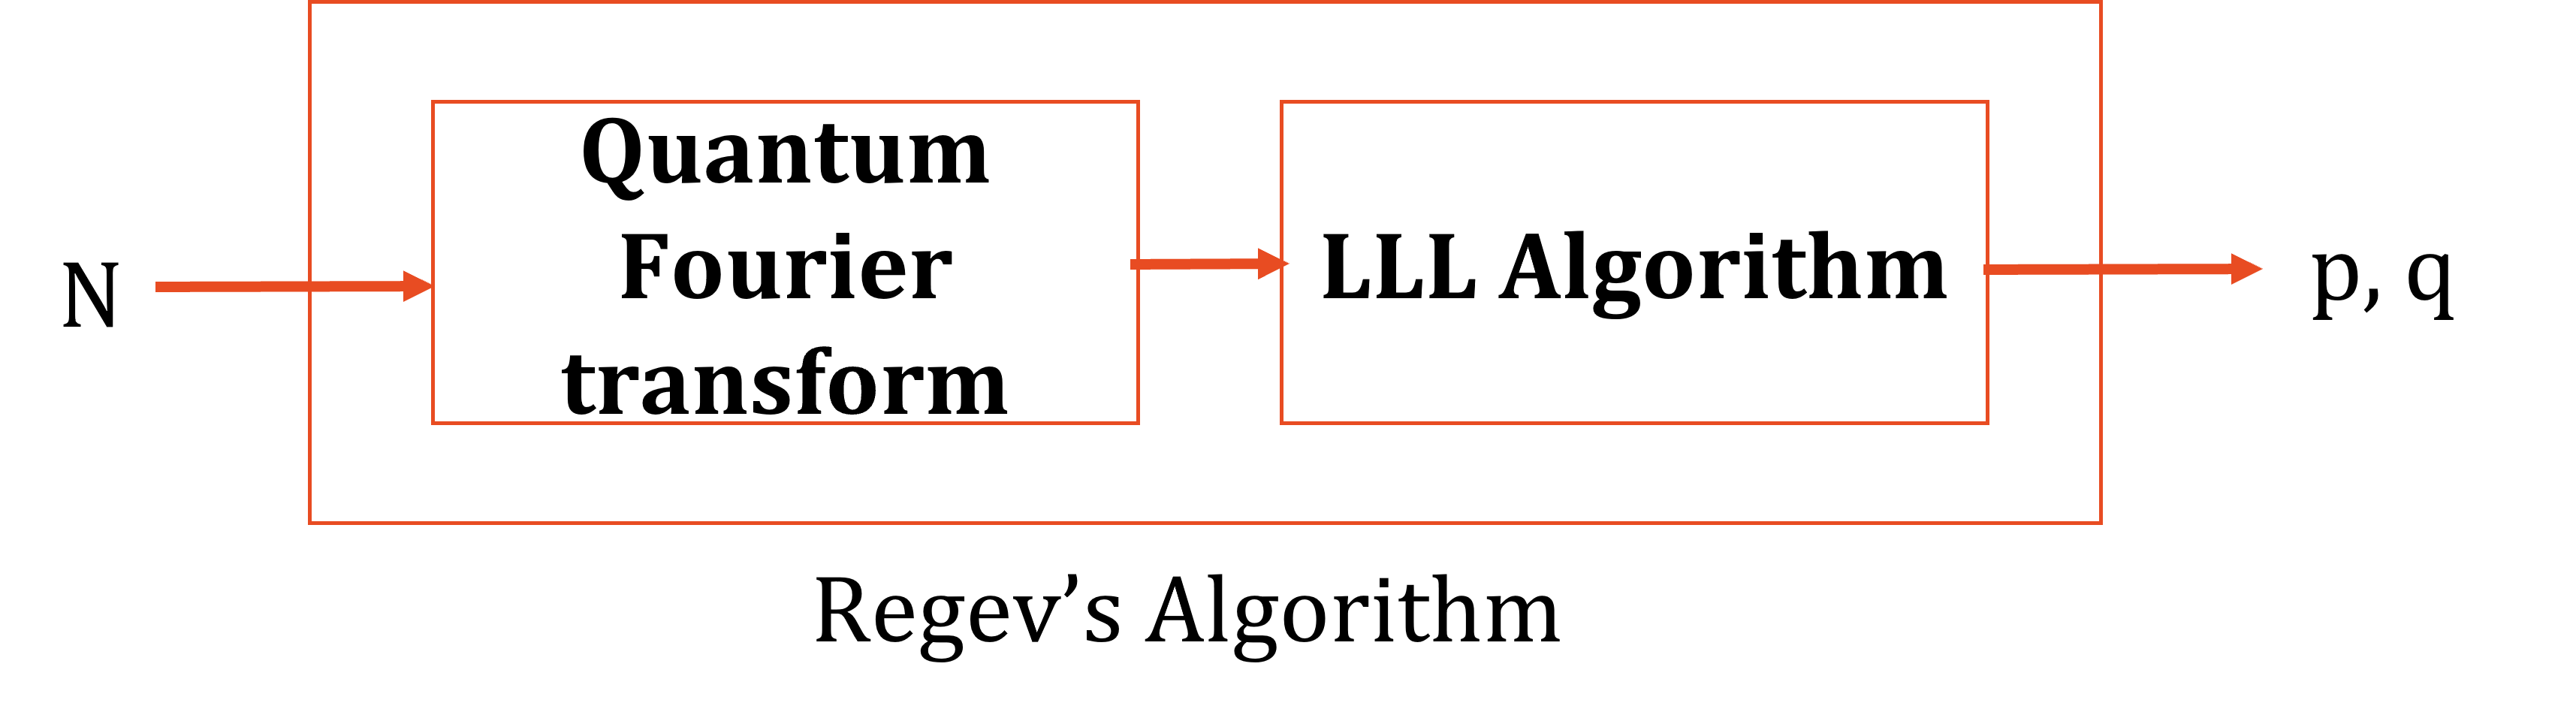
\includegraphics[width=0.75\textwidth]{pics/regev-quan-class-parts.png}
    \caption{Quantum and Classical parts in Regev's algorithm}
    \label{fig:qcma}
\end{figure}

\subsubsection{The classical post-processing}

1. $\mathsf{Lattice\ Basis\ reduction\ algorithm}$: The noisy sample $w_i=v_i+\delta_i$ is used to recover $v_i$ using the classical Lenstra–Lenstra–Lovász lattice basis reduction algorithm \cite{lenstra1982factoring}.
\vspace{1em}
2. $\mathsf{Maximum\ size\ of\ the\ sampled\ set:}$ The $\mathsf{LLL}$ algorithm has the stringent requirement that the sampled set must contain the basis-forming set for the underlying lattice. Otherwise, the algorithm will output some garbage.



\subsubsection{Abundance of the Basis Forming Sample Sets}

A lemma due to Carl Pomerance \cite{pomerance2002expected} asserts that if we uniformly sample $d+4$ elements from a group (with replacement), then it contains the basis (or generator) of the group with at least $1/2$ probability. Formally,
\begin{lemma}
    [\cite{pomerance2002expected}] Suppose that $G$ is a finite Abelian group with minimal number of generators $r$. Then, when choosing elements from $G$ independently and uniformly, the expected number of elements needed to generate $G$ is less than $r+\sigma$, where $\sigma=2.118456...$.
    \label{lemma:pom}
\end{lemma}

\begin{theorem}
    In the setting of the above lemma \ref{lemma:pom}, $r+4$ uniformly random elements of $G$ generate $G$ with probability at least $1/2$.
\end{theorem}

%%%%%%%%%%%%%%%%%%%%%%%%%%%%%%%%%%%%%%%%%%%%%%%%%%%%%%%%%%%%%%%%%%%%%%
\subsubsection{Quantum Fourier transform as quantum reduction algorithm}
%%%%%%%%%%%%%%%%%%%%%%%%%%%%%%%%%%%%
%%%%%%%%%%%%% Graphics %%%%%%%%%%%%%%%%%%
%%%%%%%%%%%%%%%%%%%%%%%%%%%%%%%%%%%%
\begin{figure}[h]
    \centering
    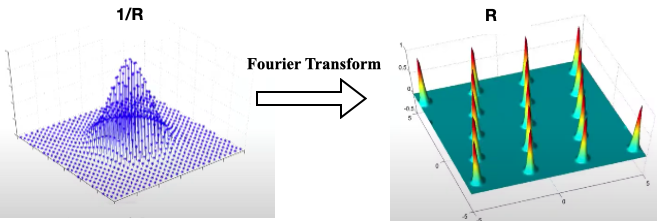
\includegraphics[width=0.75\textwidth]{pics/lattice-qft.png}
    \caption{(Fourier transform of the primal lattice to the dual lattice) $\mathsf{QFT}$ can be understood as facilitating a quantum reduction of a problem defined on the primal lattice to a problem defined on the dual lattice. The latter problem is classically easy, whereas the former is known to have no efficient classical algorithm. Note: Symbol $R$ represents the width of the associated Gaussian peaks as discussed in Subsection \ref{subsec:regev-algo}. }
    \label{fig:lattice_qft}
\end{figure}
We can interpret the role of the quantum Fourier transform as doing a quantum Turing reduction of the problem defined on the primal lattice, say problem I, to the problem defined on the dual lattice, say problem II. Problem I is to compute a non-trivial vector in the primal lattice, while problem II is to compute the basis of the primal lattice using a noisy sample vector from the dual lattice. Problem II is classically tractable, while it is unknown if Problem I is classically tractable or not. Thus, the quantum Fourier transform reduces a classically hard problem to a classically easy problem.
%%%%%%%%%%%%%%%%%%%%%%%%%%%%%%%%%%%%%%%%%%%%%%%%%%%%%%%%%%%%%%%%%%%%
\subsection{Spectral Concentration $\gamma_i$ of $\ms{GLH_i}$}\label{sec: spectral-GLH}
We recall that the definition of $\ms{GLH_i}$ includes a subset state as described below. 
\begin{prob}
    [$\ms{GLH_i}$ problem] The problem is a tuple $\Big\langle H; \ket{S};(a,b) \Big\rangle$ with the following characteristics. \newline
    $\ms{Input}$: (i) a $k$-local Hamiltonian matrix  $H=\sum_{j=1}^{m}H_j$ for an $n$-qubit system such that $\norm{H}\leq 1$, (ii) a subset state $\ket{S}\in \C^{2^n}$ of size  $\ms{|S|\leq 2^{O(log^i n)}}$ and (iii) promise gap parameter $a,\ b\in \R$ such that $|b-a|\geq \delta>0$. \newline
    $\ms{Promise}$:
    \begin{itemize}
        \item Fidelity with the ground space $\norm{\Pi_{\mathsf{gs}} \ket{S}}\geq \ms{poly(n)}$.
        \item Either case (i) $\lambda_0\leq a$ or (ii) $\lambda_0\geq b$ holds.
    \end{itemize}
    $\ms{Output}$: Output YES if $\lambda_0(H) \leq a$, and output NO if $\lambda_0(H) \geq b$.
\end{prob}
We defined the spectral concentration of an input tuple as follows.
\begin{definition}
    [Spectral concentration of a $\ms{GLH_i}$ instance] Give an instance $\Big\langle H; \ket{S};(a,b) \Big\rangle \in \ms{GLH_i}$. Its spectral concentration is defined as the inverse of the size of the set $S$. Or,
    $$\gamma_S := \frac{1}{|S|}.$$
\end{definition}
%\textbf{Remark: }Surprisingly, the problem remains $BQP$-complete even if the $2$-local Hamiltonian is restricted to any of the following families of Hamiltonians: (i) antiferromagnetic Hiesenberg model, (ii) antiferromagnetic $XY$ model on a $2D$ triangular lattice, and (iii) non-$2SLD$ Hamiltonian on a $2D$ square lattice [CFG+23].\newline
%\\

%%%%%%%%%%%%%%%%%%%%%%%%%%%%%%%%%%%%
%%%%%%%%%%%%% GRAPHIC %%%%%%%%%%%%%%
%%%%%%%%%%%%%%%%%%%%%%%%%%%%%%%%%%%%

\begin{figure}[h]
    \centering
    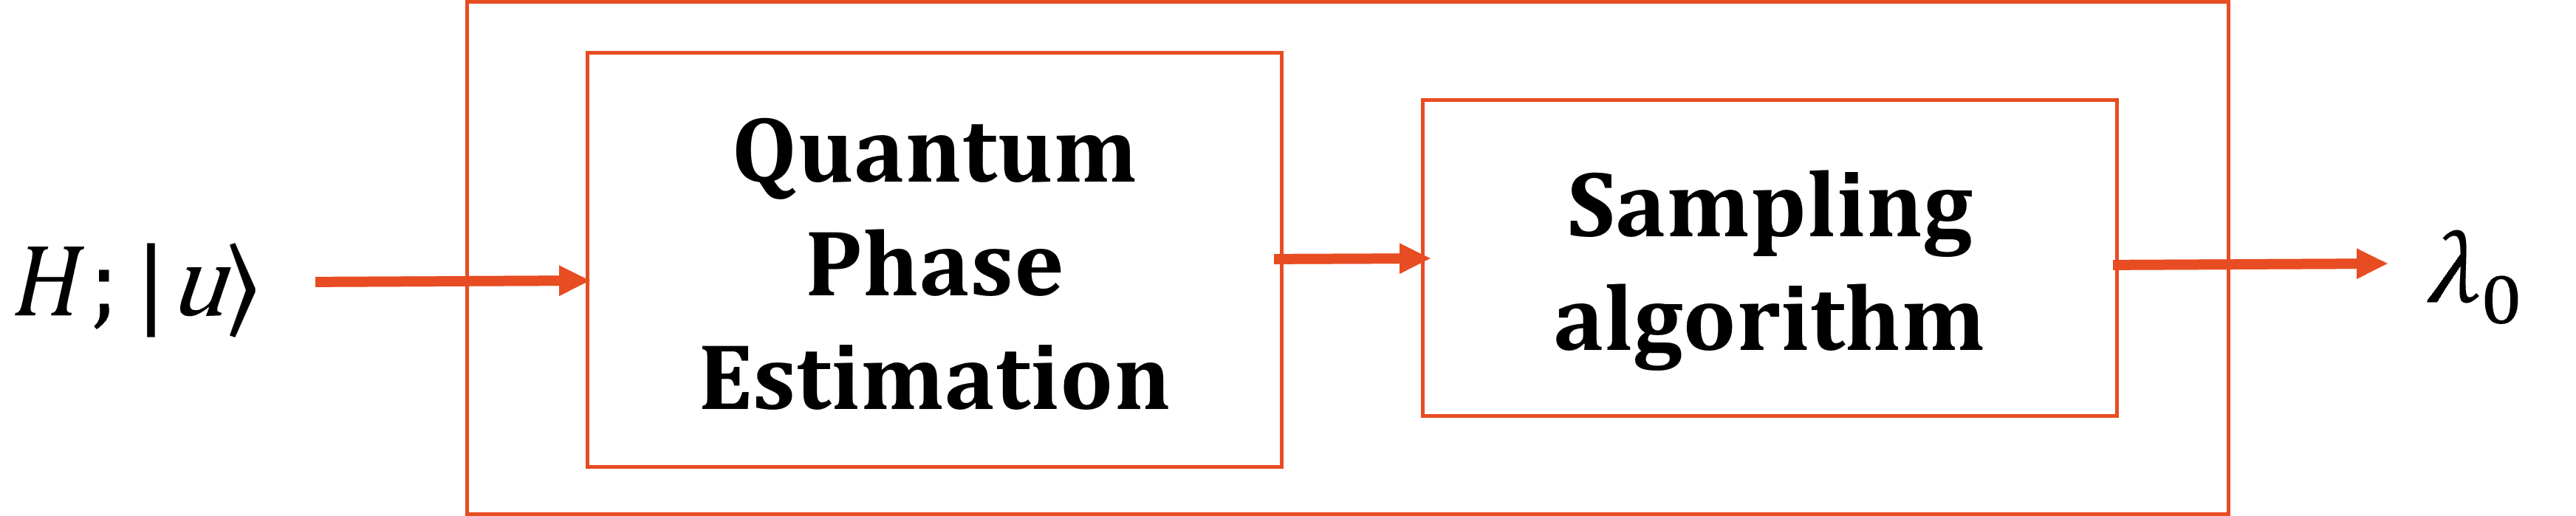
\includegraphics[width=0.75\textwidth]{pics/qpe-glh.png}
    \caption{Quantum and Classical components in the algorithm}
    \label{fig:qpe-glh}
\end{figure}

\subsubsection{The quantum algorithm}\label{subsec:qpe}
The algorithm finds the minimum eigenvalue of the given local Hamiltonian and the guided state. First, we use the quantum phase/eigenvalue estimation algorithm ($\mathsf{QPE}$) \cite{kitaev1995quantum}. $\QPE$ is run a polynomial number of times and is sampled independently. Secondly, classic post-processing on the sampled set yields the minimum eigenvalue $\lambda_0$. The formal details of the $\mathsf{QPE}$ algorithm are as follows:\newline
\\
\textbf{Remark}: The problem of estimating the phase of the unitary operator can be used to estimate an eigenvalue of the Hermitian operator due to the following lemma.\newline
\begin{theorem}
    If for a Hermitian matrix $H\in \C^{N\times N} $ and $\uu \in \C^N$, $$H\uu_i=\lambda_i\uu_i\ ;\ \ \forall i\in [N]_0  $$
then the following eigenvalue relation holds for the unitary matrix $U=e^{iH}$ $$U\uu_i=e^{i\lambda_i}\uu_i\ ;\forall i\in [N]_0 $$
\end{theorem}

\subsubsection{Quantum subroutine: quantum phase estimation $\mathsf{QPE}$}
\textbf{Context for $\QPE$:} We have a sparse unitary operator on which a controlled-$U^j$ operation can be efficiently performed for $j\in \Z$. Furthermore, we are given an eigenstate $\ket{\uu}$ of $U$ with eigenvalue $e^{2\pi i\phi_u}$. The task is to find $\tilde{\phi_u}$ such that $\norm{\tilde{\phi_u} - \phi_u}\leq \epsilon$.\newline
\\

%%%%%%%%%%%%%%%%%%%%%%%%%%%%%%%%%%%%
%%%%%%%%%%%%% GRAPHIC %%%%%%%%%%%%%%%%%
%%%%%%%%%%%%%%%%%%%%%%%%%%%%%%%%%%%%

\begin{figure}[h]
    \centering
    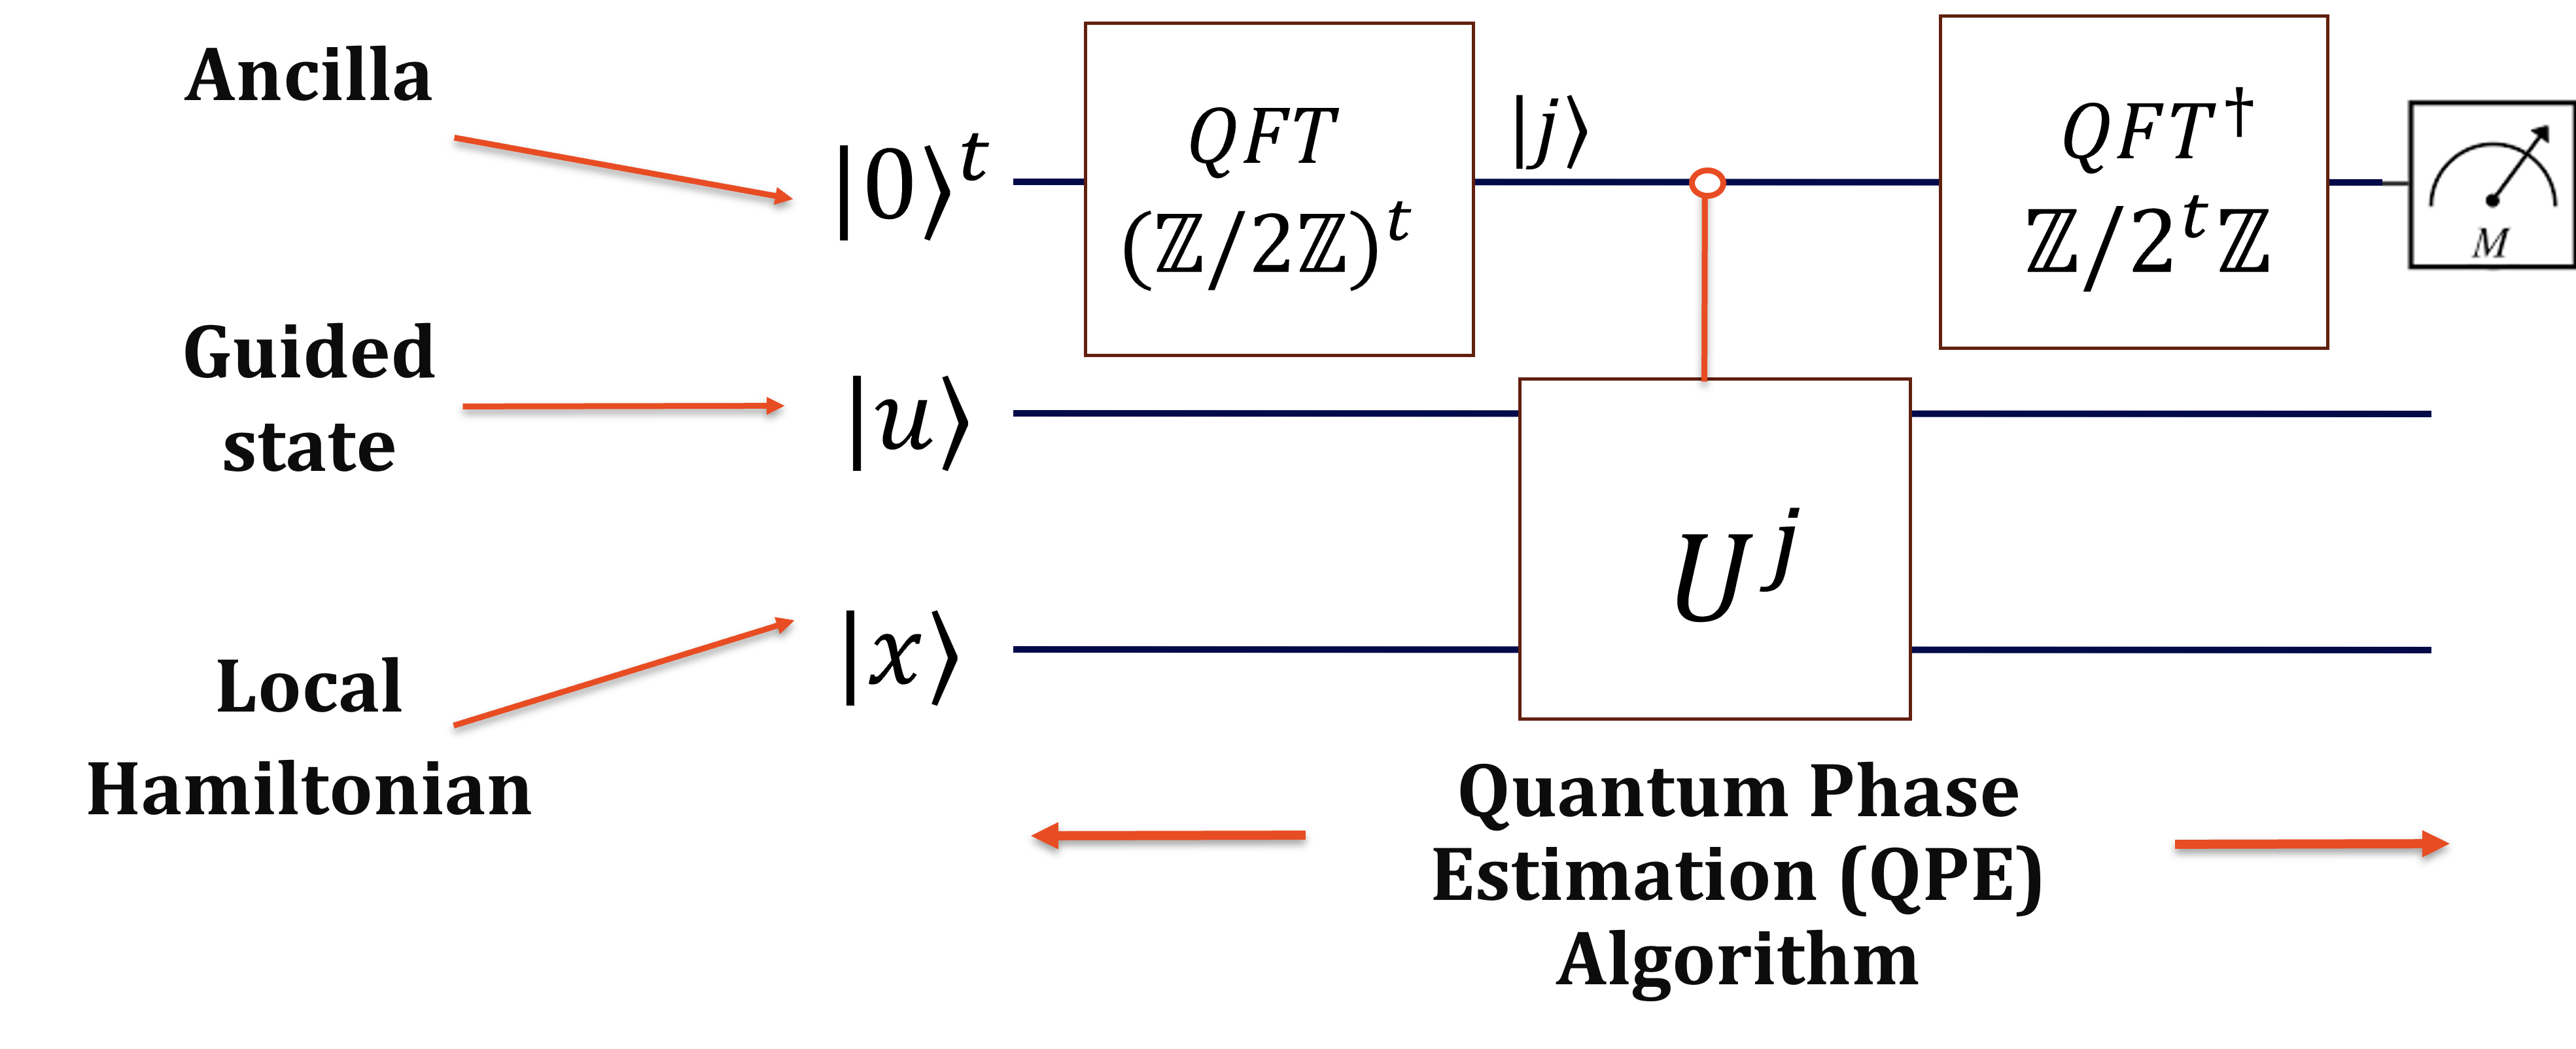
\includegraphics[width=0.75\textwidth]{pics/UQA_circuit.png}
    \caption{(Quantum Phase/Eigenvalue Estimation) A guided state $\ket{\uu}$ and the description of the local Hamiltonian \textbf{x} is provided as input. The unitary $U=e^{i{\xx}}$. Two different types of quantum Fourier transform have been employed: (i) a quantum Fourier transform over the  Boolean group $(\Z/2\Z)^2$, also called the Hadamard transform, and (ii) a quantum Fourier transform over the group $\Z/2^n\Z$.}
    \label{fig:qpe}
\end{figure}


\subsubsection{Algorithmic Procedure for $\mathsf{QPE}$}
1. Prepare the initial state: $$\ket{0}^m\ket{\uu}\ket{\xx}$$
2. Create the superposition: $$\ket{0}^m\ket{\uu}\ket{\xx} \rightarrow  \frac{1}{\sqrt{2^m}} \sum_{j=0}^{2^m-1}\ket{j}\ket{\uu}\ket{\xx}$$
3. Apply controlled-$U^j$: $$\frac{1}{\sqrt{2^m}} \sum_{j=0}^{2^m-1}\ket{j}\ket{\uu}\ket{\xx} \rightarrow \frac{1}{\sqrt{2^m}} \sum_{j=0}^{2^m-1}\ket{j}U^j\ket{\uu}\ket{\xx}= \frac{1}{\sqrt{2^m}} \sum_{j=0}^{2^m-1}e^{2\pi ij\phi_u}\ket{j}\ket{\uu}\ket{\xx}$$
4. Apply the inverse Fourier transform: $$ \frac{1}{\sqrt{2^m}} \sum_{j=0}^{2^m-1}e^{2\pi ij\phi_u}\ket{j}\ket{\uu}\ket{\xx} \rightarrow \ket{\phi_u}\ket{\uu}\ket{\xx}$$
5. Measure the first register and output the number: $$ \ket{\phi_u}\ket{\uu}\ket{\xx} \rightarrow \tilde{\phi_u}$$
\subsubsection{Resource and running time analysis for $\mathsf{QPE}$}

\begin{lemma}
    Quantum eigenvalue estimation lemma: Let $\mathsf{H=\sum_{i=1}^{m}H_i}$ be a $2$-local Hamiltonian acting on $n$ qubits, with eigenvectors $|\psi_j\rangle$ and the corresponding eigenvalues $\lambda_j\in [0,1]$. Then there is a quantum circuit that, given an input eigenvector $\ket{\psi_j}$, will output (with probability $\geq p$) an $\epsilon$-approximation of $\lambda_j$ (that is, $\tilde{\lambda_j}$ such that $|\tilde{\lambda_j}-\lambda_j|\leq \epsilon$). The depth of the quantum circuit is 
    \begin{equation}
        d \leq \mathsf{poly\Big( m,\frac{1}{\epsilon},\frac{1}{p}\Big)}.
    \end{equation}
\end{lemma}

%For detailed analysis and proof of correctness, see section \ref{subsec:QPE}. 
\subsubsection{Classical subroutine: the sampling algorithm} 
Each measurement of $\QPE$ gives an eigenvalue of the input Hamiltonian. Since our goal is to find the minimum eigenvalue, we need to collect a sufficiently large sample to ensure it contains the minimum eigenvalue with high probability. Thus, we need to run the $\QPE$ circuit multiple times. The upper bound on the repetition of $\QPE$ is estimated using the following theorem.
\begin{theorem}
    The maximum number of times the $\QPE$ algorithm needs to be repeated to get a sample set from which $\lambda_0$ (min. eigenvalue) can be extracted with the probability of $1/2+\delta_p$ is $$O\big(\mathsf{log}(1/\delta_p)\big).$$
\end{theorem}
\textbf{Proof:} Since the probability of getting $\lambda_0$ in the first trial is greater than $\gamma$. Then, $$\textrm{Pr}[\textrm{Not \ getting $\lambda_0$ in the first trial}]\leq 1-\frac{1}{\gamma}$$
Similarly,
$$\textrm{Pr}[\textrm{Not \ getting $\lambda_0$ in the $t$-th trial}]\leq 1-\Big(\frac{1}{\gamma}\Big)^t$$ As per our requirement, we want 
\begin{equation}
    1-\Big(\frac{1}{\gamma}\Big)^t\geq \frac{1}{2}+\delta_p \implies \frac{1}{2}-\delta_p \geq \Big(\frac{1}{\gamma}\Big)^t.
\end{equation}
\begin{equation}
    t\leq \frac{\log \Big(\frac{1}{2}-\delta_p \Big)}{\log \frac{1}{\gamma}}.
\end{equation}


%%%%%%%%%%%%%%%%%%%%%%%%%%%%%%%%%%%%%%%%%%%%%%%%%%%%%%%%%%
%%%%%%%%%%%%%%%%% SPECTRAL INTERPRETATION %%%%%%%%%%%%%%%%
%%%%%%%%%%%%%%%%%%%%%%%%%%%%%%%%%%%%%%%%%%%%%%%%%%%%%%%%%%

\subsubsection{The Spectral Density Analysis}
%%%%%%%%%%%%%%%%%%%%%%%%%%%%%%%%%%%%
%%%%%%%%%%%%% GRAPHIC %%%%%%%%%%%%%%
%%%%%%%%%%%%%%%%%%%%%%%%%%%%%%%%%%%%

\begin{figure}[h]
    \centering
    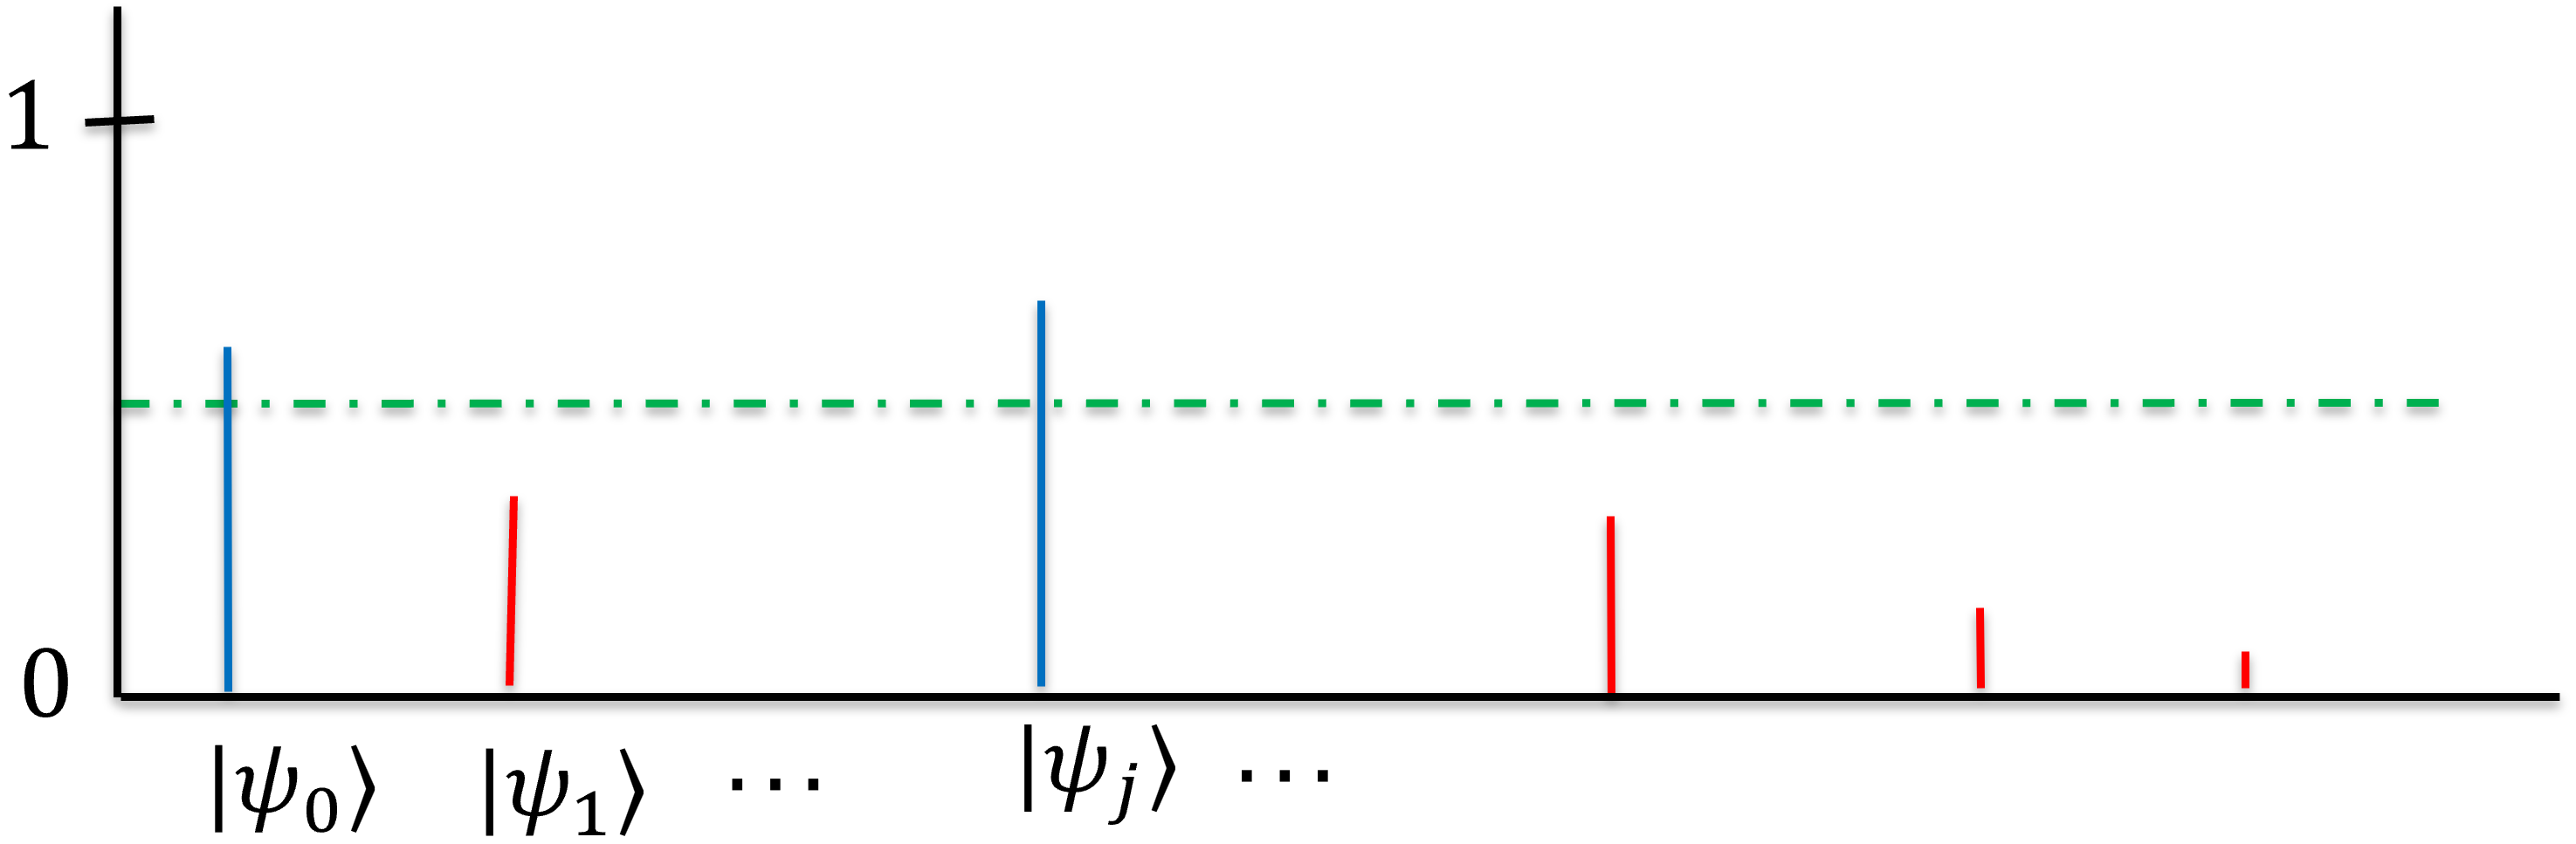
\includegraphics[width=0.75\textwidth]{pics/overlap-u-psi.png}
    \caption{   (Spectral interpretation) The Height of a peak represents the fidelity of the guided state with an eigenstate of the Hamiltonian $H$. The blue peaks crossing above the horizontal green line correspond to the eigenstates that have substantial overlap with the guided state. The eigenvalue associated with these 'blue' eigenstates will appear more frequently in the sample collected via the QPE algorithm.}
    \label{fig:spec-thres}
\end{figure}

Due to the spectral theorem, any Hermitian matrix $H\in \C^{N\times N}$ can be decomposed into its eigenbasis as:
$$H=\sum_{i=0}^{N-1}\lambda_i\ket{\psi_i}\bra{\psi_i}$$
For any normalized vector $\ket{\uu} \in \C^N $,  the $\mathsf{spectral\ measure}$ induced by the matrix $H$ and the vector $\ket{\uu}$ is a probability distribution on the spectrum of $H$ such that the probability of getting eigenvalue $\lambda_i$ occurs with 
\begin{equation}
    \mathsf{Pr[measuring\ \lambda_i]} \geq | \langle \psi_i|\uu\rangle|^2.
\end{equation}
Typically, we don't have direct access to the ground state of a Hamiltonian; instead, we have access to a state that overlaps with it. However, this can be used to compute the minimum eigenvalue with a success probability depending on the extent of the overlap.
%%%%%%%%%%%%%%%%%%%%%%%%%%%%%%%%%%%%%%%%%%%%%%%%%%%%%%%%%%%%%%%%%%%%%%%%%%%%%%%%%%%%%%%%%%%%%%%

\begin{lemma}
    Suppose we have been given a state 
    \begin{equation}
        \ket{\uu} = \sum_{i=0}^{N-1} \alpha_{i} \ket{\psi_i}
    \end{equation}
    instead of the ground state $\ket{\psi_0}$ for computing  using the $\QPE$ algorithm. Then the probability of measuring $\lambda_0(H)$ when the input to the $\mathsf{QPE}$ is $(H,\ \ket{\uu})$ is lower bounded by 
    \begin{equation}
        \mathsf{Pr[measuring\ \lambda_i]} \geq |\alpha_0|^2(1-\epsilon)
    \end{equation}
    where $(1-\epsilon)$ is the probability of success of the phase estimation.

\end{lemma}

\subsubsection{Abundance of low-energy states and the success probability of $\mathsf{QPE}$ }
$\mathsf{QFT}$ plays the role of a change of basis from a standard basis to the eigenbasis of the Hamiltonian matrix. The standard basis consists of the set $\mathcal{B}=\{\ket{\zz} |\ \zz \in \{0,1\}^n\}$ while the set of eigenbasis of the Hamiltonian $H$ is the set $\mathcal{E}=\{\ket{\psi}\ |\ H\ket{\psi}=\lambda\si; \si \in {\R^{2^n}} \}$.\par Stroeks et al. have shown that if the guiding state has good overlap with the $\mathsf{O(1)}$ eigenstates, then there is a randomized algorithm to solve the guided local Hamiltonian problem. We propose a new variant of the guided local Hamiltonian problem that quantifies the number of eigenstates with good overlap with the guiding vector as a computational resource.
%%%%%%%%%%%%%%%%%%%%%%%%%%%%%%%%%%%%%%%%%%%%%%%%%%%%%%%%%%%%%%%%
\subsection{An Algorithm to Estimate $\gamma_i$}\label{sec: algo}
\subsubsection{Relating Guidance Value and Quantum Circuit Depth}\label{subsec:circ-depth-uqa}
%%%%%%%%%%%%%%%%%%%%%%%%%%%%%%%%%%%%
%%%%%%%%%%%%% GRAPHIC %%%%%%%%%%%%%%
%%%%%%%%%%%%%%%%%%%%%%%%%%%%%%%%%%%%
\begin{comment}
    \begin{figure}[h]
    \centering
    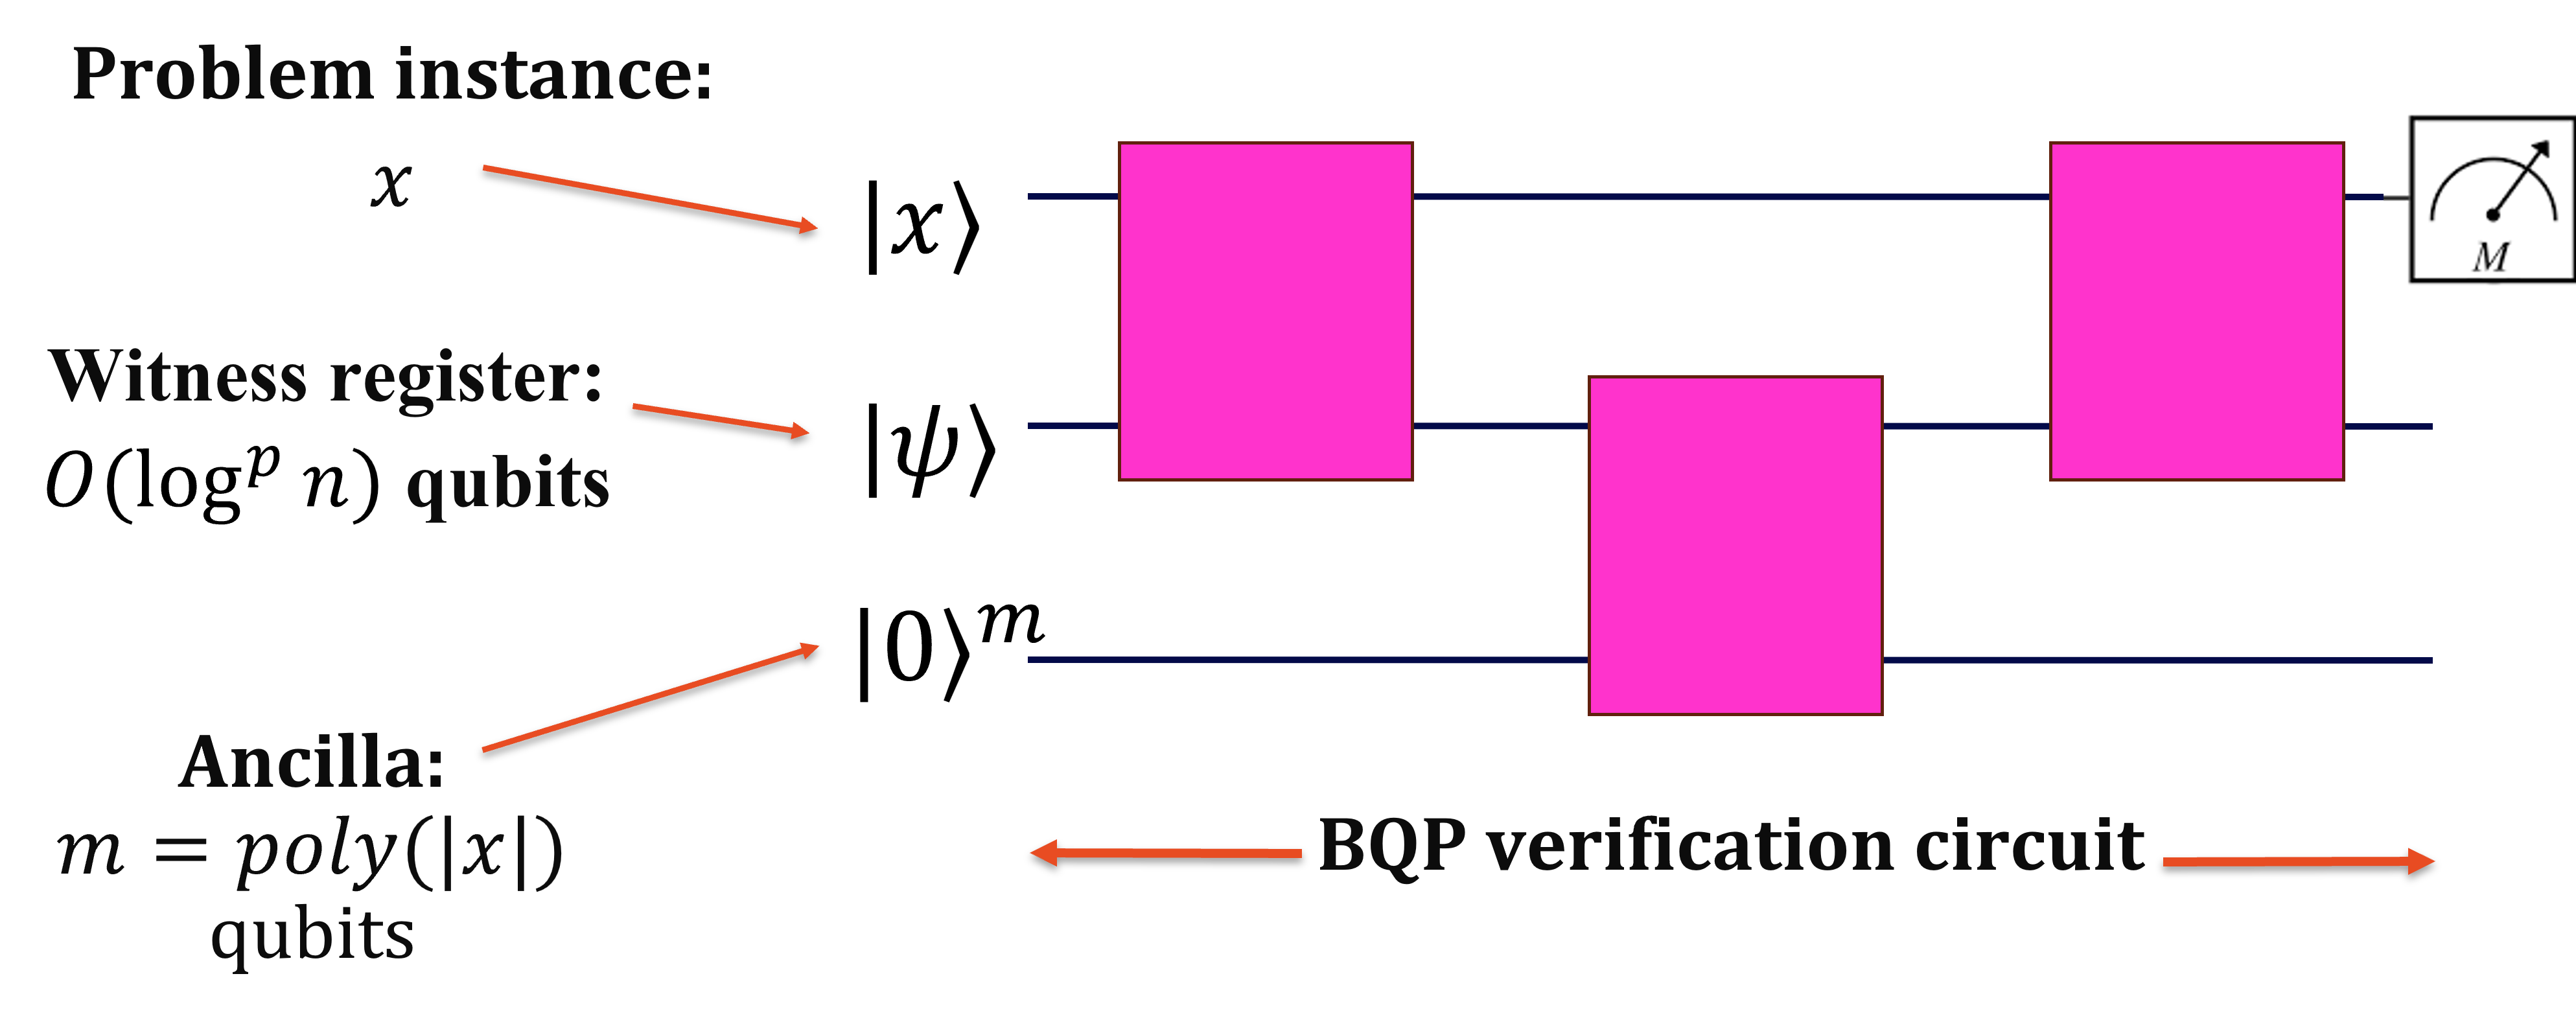
\includegraphics[width=0.75\textwidth]{pics/verif-logn-witness.png}
    \caption{QCMA verification circuit}
    \label{fig:qcma}
\end{figure}
\end{comment}
%%%%%%%%%%%%%%%%%%%%%%%%%%%%%%%%%%%%%%%%

It is anticipated that a problem with a higher guidance value will be solved using a relatively shallow quantum circuit compared to a problem with a lower guidance value. Now, we will precisely quantify the dependency of guidance value ($\gamma$) on circuit depth ($d(n)$) through the following analysis.

\begin{theorem}
    There exists a method to generate a guided state $\ket{\uu}$ such that the value of the guidance parameter scales as \begin{equation}
        \gamma:=|\langle \uu \ket{\psi_{\hist}}|^2 \geq \frac{N}{d(n)+N+1}.
    \end{equation}
    where, $N=O(d(n))$.
\end{theorem}

Proof: It follows from the hardness result for the $\ms{GLH_i}$ problem for the class $\beta_p$-$\QCMA$. The key observation is that, in the worst-case scenario, the maximally mixed state is the optimal choice as the guiding state. It has the following practical corollaries of interest.
\begin{coro}
    If $d(n)= \mathsf{poly(n)}$, then there exists a guiding state $\ket{\uu}$ with
    $$\gamma:=|\langle \uu \ket{\psi_{\hist}}|^2 \geq \frac{1}{\poly(n)}.$$
\end{coro}

\begin{coro}
    If $d(n)= 2^{c \cdot \mathsf{log}^p(n)}$, then there exists a guiding state $\ket{\uu}$ with
    $$\gamma:=|\langle \uu \ket{\psi_{\hist}}|^2 \geq \frac{1}{2^{{\polylog}(n)}}.$$
\end{coro}

\begin{coro}
    If $d(n)= 2^{\poly(n)}$, then there exists a guiding state $\ket{\uu}$ with
    $$\gamma:=|\langle \uu \ket{\psi_{\hist}}|^2 \geq \frac{1}{ 2^{\poly(n)} }.$$
\end{coro}




%%%%%%%%%%%%%%%%%%%%%%%%%%%%%%%%%%%%%%%%%%%%%%%%%%%%%%%%%%%%%%%
\subsection{Relating $\gamma_i$ to level $i$ of $\ms{QMAH}$ }
%%%%%%%%%%%%%%%%%%%%%%%%%%%%%%%%%%%%%%%%%%%%%%%%%%%%%%%%%%%%%%%%%%%%%%%%%%%%%%%%%%%%%%%%%%%%%%%%%%%%%%%%%%%%%%%%%
%\subsubsection{Classically and Quantumly tractable cases of $k$-$\mathsf{LH}$ problems}
We present two criteria under which some variant of $\mathsf{LH}$ problems are either classically or quantumly easy. This will illustrate why the presence of certain types of Pauli (string) Hamiltonians\footnote{The matrix $\mathsf{Z_1\otimes Z_2 \otimes I_3 \otimes I_4 \otimes Z_5}$ is a five-qubit Pauli (string) Hamiltonian with the Pauli degree three.} with degree $d\leq 2$  with a frequency less than a certain threshold is tractable. This will help build intuition and the proof of correctness.\newline
\textbf{Classically tractable case:} For the classically tractable case, we start with the one local Hamiltonian, which is known to be in $\mathsf{P}$.
\begin{prob}
    [$\mathsf{\{X,\ Y,\ Z\}}$-$\mathsf{Hamiltonians}$] $\mathsf{Input}$: A one local Hamiltonian on $n$-qubit system which takes the following form 
    \begin{equation}
        \mathsf{H= \sum_{k\in [n]}\alpha_k X_k +\beta_k Y_k + \gamma_k Z_k} 
    \end{equation}
    $\mathsf{Promise}:$ Either, (i) $\mathsf{\lambda_0(H)}\leq a$, or (ii) $\mathsf{\lambda_0(H)\geq b}$. Along with the promise gap of $\mathsf{b-a \geq 1/poly(n)}$. 
    \label{thm:z-ham} 
\end{prob}
A polynomial-time algorithm exists for the problem. We mention it for completeness.
\begin{theorem}
    $1$-$\mathsf{Local\ Hamiltonian}$ is in $\mathsf{P}$.
\end{theorem}
$\mathsf{Proof}$: There are two methods to construct this. First, construct the ground state, which is guaranteed to be a product state over $n$ qubits.
\begin{equation}
    \ket{\psi}= \bigotimes_{i=1}^n \ket{\psi_i}
\end{equation}
Now, each one-particle state $\ket{\psi_i}$ can be identified, which minimizes the associated 1-local Hamiltonian terms (in which the $i$th particle participates). Each qubit can be present in a maximum of three clauses/terms. Thus, we need to run the checking process at most a polynomial number of times.\footnote{\textbf{Note}: the same technique won't help give a polynomial time algorithm for the 2-Local Hamiltonian problem. The reason is that each qubit might share a clause/term with $(n$-$1)$ other qubits. The same method would require an exponential number of checks, in the worst case.}    \par
The second proof evokes a result from matrix theory. For 1-local Hermitian matrices, there always exists a 1-qubit unitary matrix  $ \mathsf{U_{2\times 2}}$ such that they $\mathsf{U^{\otimes n}}$ can simultaneously diagonalize the input 1-Local Hamiltonian $\mathsf{H}$. Once diagonalized, one can easily find the minimal eigenvalue by inspecting the minimum of the diagonal entries. \qed 

Next, we introduce an $\mathsf{NP}$-$\mathsf{complete}$ version of $2$-local Hamiltonian problem due to \cite{Bar82}. The reason for the Hardness is due to the appearance of $\mathsf{Complexity\ generator}$ terms in high frequency. 
\begin{prob}
    [$\mathsf{\{ZZ, \ Z\}}$-$\mathsf{Hamiltonians}$] $\mathsf{Input}$: A two local Hamiltonian on $n$-qubit system which takes the following form 
    \begin{equation}
        \mathsf{H=\sum_{i,k\in [m]}\alpha_{i,j}Z_i \otimes Z_j + \sum_{k\in [n]}\beta_k Z_k} 
    \end{equation}
    $\mathsf{Promise}:$ Either, (i) $\mathsf{\lambda_0(H)}\leq a$, or (ii) $\mathsf{\lambda_0(H)\geq b}$. Along with the promise gap of $\mathsf{b-a \geq 1/poly(n)}$.
    \label{prob:zz-ham}
\end{prob}

The problem is $\NP$-complete if the parameter $\mathsf{m=poly(n)}$. We prove that the problem is in $\mathsf{P}$ if we restrict the parameter.

\begin{theorem}
The problem \ref{prob:zz-ham} is in $\mathsf{P}$ if parameter $\mathsf{m=O(log(n))}$. \label{thm:zz-ham}
\end{theorem}

$\mathsf{Proof:}$ The complexity of the problem is due to the appearance of the $\mathsf{Z_i\otimes Z_j}$ terms in the Hamiltonian. We (informally) call it classical $\mathsf{complexity\ generating}$ terms. The 1-local term does not add to the complexity. Restricting the parameter $\mathsf{m=O(log(n))}$ implies the number of variables appearing in $\mathsf{complexity\ generating}$ terms is not too large. Thus, the search space is upper bounded by $\mathsf{poly(n)}$. The reason is that the number of possible basis states/assignments over $\mathsf{m=O(log(n))}$ many qubits/variables is $\mathsf{2^{m} = poly(n)}$. Therefore, one can check each $\mathsf{m=O(log(n))}$ possibility, where each check will require at most $\mathsf{poly(n)}$ time.\footnote{This brute force algorithm can be enhanced by using a randomized algorithm like the method similar to Schroning's $\SAT$ algorithm. This will result in a polynomial speed-up over the brute-force method. In practical cases, this polynomial speed-up might be helpful.} It should be noted that the one-local Hamiltonian can be managed using the strategy employed in the polynomial-time algorithm for the 1-local Hamiltonian problem.  \qed 

Assuming Exponential Time Hypothesis for $\SAT$ is true, we can prove that there is \textbf{no} classical algorithm for problem \ref{thm:zz-ham} with sub-exponential running time, that is, any algorithm for $3$-$\SAT$ must take $\mathsf{O^{*}(2^{\delta n}})$ time for $\delta>0$. The notation $\mathsf{O^{*}}$ indicates the suppression of $\poly(n)$ factor as it will get asymptotically dominated by the exponential function. \textbf{Note}: The result implies the worst-case analysis of the problem, or one can create an instance for which any polynomial-time algorithm is unlikely to succeed (assuming ETH is true.) 
\begin{theorem}
    If the Exponential Time Hypothesis is true, then there is no polynomial time algorithm for $\mathsf{\{ZZ,Z\}}$-$\mathsf{HAMILTONIAN}$  on $n$-qubits for $\mathsf{m=O(log^p n)}$ with $\mathsf{p>1}$. \label{thm:ETH}
\end{theorem}
$\mathsf{Proof:}$ The proof strategy is to show any algorithm for $\SAT$ that saturates the upper bound prescribed by $\mathsf{ETH}$, then the same algorithm can only yield a superpolynomial algorithm for the case when $\mathsf{m=O(log^{p} n)}$, for any $p>1$. We evoke the known $\poly(n)$-time and $\mathsf{O(n)}$-space reduction of $3\SAT$ to $\mathsf{MAX2SAT}$. Also, there is  $\poly(n)$-time and $\mathsf{O(n)}$-space reduction of $\mathsf{MAX2SAT}$ to $\mathsf{\{ZZ,Z\}}$-$\mathsf{HAMILTONIAN}$ (\ref{prob:zz-ham})  problem. \par
As per $\mathsf{ETH}$, $3\SAT$ over $n$-variables would require at most $\mathsf{O^{*}(\alpha^{n})}$ computational steps (for $\alpha \in (1,2]$). When the number of clauses is $\mathsf{m=O(log^{1+\epsilon} n)}$, then in the worst-case scenario, we can have $\mathsf{3m}$ variables (3 variables per clause). Thus, it would require at most 
\begin{equation}
    \mathsf{T(n)=\alpha^{3 \cdot log^{1+\epsilon} n}}
\end{equation}
computational steps. Thus, for any $\epsilon>0$, it would require a super-polynomial number of steps, in the worst case. Since the reduction of $3\SAT$ to $\mathsf{\{ZZ, Z\}}$-$\mathsf{HAMILTONIAN}$  causes linear blow-up in terms of the number of variables, the above derived time bound for restricted $3\SAT$ is translated to restricted $\mathsf{\{ZZ,  Z\}}$-$\mathsf{HAMILTONIAN}$ too. 
\qed

\subsubsection{Quantumly tractable case}
The above analysis has a quantum counterpart as follows. 
\begin{prob}
    [$\mathsf{\{XX,YY,ZZ,\ X,Y,Z\}}$-$\mathsf{Hamiltonians}$] $\mathsf{Input}$: A two local Hamiltonian on $n$-qubit system which takes the following form 
    \begin{equation}
        \mathsf{H=\sum_{i,k\in [m]}\alpha_{i,j}X_i \otimes X_j + \beta_{i,j} Y_i \otimes Y_j + \gamma_{i,j}Z_i \otimes Z_j+ \sum_{k\in [n]}a_k X_k +b_k Y_k + c_k Z_k} 
    \end{equation}
    $\mathsf{Promise}:$ Either, (i) $\mathsf{\lambda_0(H)}\leq a$, or (ii) $\mathsf{\lambda_0(H)\geq b}$. Along with the promise gap of $\mathsf{b-a \geq 1/poly(n)}$.
    \label{prob:xyz-ham}
\end{prob}
The problem is $\mathsf{QMA}$-complete if the parameter $\mathsf{m=poly(n)}$ \cite{CM16}. We prove the problem is in $\mathsf{BQP}$ if we restrict the parameter $\mathsf{m=O(log(n))}$. 
\begin{theorem}
The problem \ref{prob:xyz-ham} is in $\mathsf{BQP}$ if parameter $\mathsf{m=O(log(n))}$. \label{thm:xyz-ham}
\end{theorem}
$\mathsf{Proof:}$ The complexity of the problem is due to $\mathsf{X_i \otimes X_j + Y_i \otimes Y_j + Z_i \otimes Z_j}$ terms in the Hamiltonian. We (informally) call it quantum $\mathsf{complexity}$ $\mathsf{generating}$ terms. As in the classical case, the 1-local terms do not increase the complexity. There is a subtle difference between the proof for this case and the classical counterpart. Our algorithm is inspired by the proof of $\mathsf{QMA_{log} = BQP}$ \cite{marriott2005quantum}. The idea is to run the Quantum phase estimation algorithm on a maximally mixed state over $\mathsf{m=O(log(n))}$ qubits. The qubits on which only a 1-local Hamiltonian acts can be managed using the strategy employed in the polynomial-time algorithm for the 1-local Hamiltonian problem. \qed \newline
Theorems \ref{thm:zz-ham} and \ref{thm:xyz-ham} equip us with a critical characterization, in terms of Pauli string Hamiltonian, for terms whose appearance till a specific frequency makes the input instance tractable. This is sufficient to bring the notion of Fourier analysis, over bounded Hermitian operators, to be an essential tool to design a spectrally-inspired $\mathsf{GENERATE\ GS}$ algorithm. \newline

\subsubsection{What if parameter $\mathsf{m > O(log(n))}$?} \label{heuristics}
Assuming some hardness assumption like $\BQP\neq \QCMA$ and Exponential Time Hypothesis for $\SAT$ and $k$-$\LH$, our ground state algorithm can be proved to be optimal in the worst case scenario for $\mathsf{m = O(log^p(n))}$ where $p>1$. Yet, we have identified some cases in this regime where a polynomial-time algorithm can be provided under specific criteria. We list them as follows.
(To be updated)

%%%%%%%%%%%%%%%%%%%%%%%%%%%%%%%%%%%%%%%%%%%%%%%%%%%%%%%%%%%%%%%%%%
\begin{comment}
    \begin{tikzpicture}[node distance=2cm]

\node (start) [startstop] {2-Local Hamiltonian};
\node (in1) [io, below of=start] {Pauli Normal Form};
\node (pro1) [process, below of=in1] {Checking Types of Pauli Terms};
\node (dec1) [decision, below of=pro1, yshift=-0.5cm] {Decision 1};

\node (pro2a) [process, below of=dec1, yshift=-0.5cm] {Process 2a
text text text text
text text text 
text text text};

\node (pro2b) [process, right of=dec1, xshift=2cm] {Process 2b};
\node (out1) [io, below of=pro2a] {Output};
\node (stop) [startstop, below of=out1] {Stop};

\draw [arrow] (start) -- (in1);
\draw [arrow] (in1) -- (pro1);
\draw [arrow] (pro1) -- (dec1);
\draw [arrow] (dec1) -- node[anchor=east] {yes} (pro2a);
\draw [arrow] (dec1) -- node[anchor=south] {no} (pro2b);
\draw [arrow] (pro2b) |- (pro1);
\draw [arrow] (pro2a) -- (out1);
\draw [arrow] (out1) -- (stop);

\end{tikzpicture}
\end{comment}



%%%%%%%%%%%%%%%%%%%%%%%%%%%%%%%%%%%%%%%%%%%%%%%%%%%%%%%%%%i
\begin{comment}
    %%%%%%%%%%%%%%%%%%%%%%%%%%%%%%%%%%%%%%%%%%%%%%%%%%%%%%%%%%%%%%%%%%
\begin{figure}[h]
    \centering


    \begin{forest}
    important/.style={name=#1,draw={red,thick}}
    [2-Local Hamiltonian, s sep=2mm, for tree={fill=orange, draw}
        [Pauli Normal Form, for tree={fill=yellow}
            [1-Local Pauli, for tree ={fill = green!30}
                [Tractable (\ref{thm:z-ham}), for tree={fill=green}]
            
            ]
            [2-Local Pauli, for tree={fill = yellow}
                [\{ZZ\} Pauli Terms, for tree={fill=yellow}
                    [$m \leq \mathsf{O{(log (n))}}$, for tree={fill=green!30} 
                        [Tractable (\ref{thm:zz-ham}),for tree={fill=green}]
                    ]
                    [$m \geq \mathsf{O{(log (n))}}$, for tree={fill=red!20}
                        [Case I, for tree={fill=green!30}
                            [Tractable (\ref{heuristics}), for tree={fill=green}]
                        ]
                        [Case II, for tree={fill=red!50}
                            [Intractable, for tree= {fill=red}]
                        ]
                    ]
                ]
                
                [\{XX + YY+ ZZ\} Pauli, for tree={fill=yellow}
                    [$m \leq \mathsf{O{(log (n))}}$, for tree={fill=green!30} 
                        [Tractable (\ref{thm:xyz-ham}),for tree={fill=green}]
                    ]
                    [$m \geq \mathsf{O{(log (n))}}$, for tree={fill=red!20} 
                        [Case I, for tree={fill=green!30}
                            [Tractable (\ref{heuristics}), for tree={fill = green}]
                        ]
                        [Case II, for tree={fill=red!50}
                            [Intractable, for tree={fill = red}]
                        ]
                    
                    ]
                        
                ]
            ]
        ]
    ]
    \measurexdistance[\texttt{s sep(root)}=#1]
        {(left.north east)}{(right.north west)}{(.north)+(0,3mm)}{above}
\end{forest}

    \caption{Flow chart to design the ground state for a 2-local Hamiltonian problem. The parameter $m$ represents the frequency of quantum and/or classical $\mathsf{complexity\ generator}$ terms, that is, $\mathsf{\{ZZ\}}$ and/or $\mathsf{\{XX+YY+ZZ\}}$ terms. It also depicts the worst-case performance of the Local Hamiltonian algorithms when applied to the ground state prepared by our method.}
    \label{fig:pauli-normal-form}
\end{figure}
\end{comment}
%%%%%%%%%%%%%%%%%%%%%%%%%%%%%%%%%%%%%%%%%%%%%%%%%%%%%%%%%%%%%%%
%\subsection{Characterizing $\ms{QMAH_i}$ through concentration}
%(To be updated)
%\newpage
%%%%%%%%%%%%%%%%%%%%%%%%%%%%%%%%%%%%%%%%%%%%%%%%%%%%%%%%%%%%%%%
%%%%%%%%%%%%%%%%%%%%%%%%%%%%%%%%%%%%%%%%%%%%%%%%%%%%%%%%%%%%%%%
%%%%%%%%%%%%%%%%%%%%%%%%%%%%%%%%%%%%%%%%%%%%%%%%%%%%%%%%%%%%%%%%%
\section{A $\ms{poly}(\gamma_i$) algorithm for $\ms{GLH}_i$ }\label{sec: main-algo}
\subsection{The algorithm}\label{sec:uqa}
We introduced this parametrized version of the $\ms{GLH_i}$ problem in the section \ref{prob: beta-GaLH}. Since the problem lies in $\ms{QMAH}_i$, it is unlikely to have a polynomial-time quantum algorithm. At the same time, it is unlikely to be as difficult as $\ms{QMAH}_i$-$\mathsf{complete}$\footnote{Please note, the best known quantum algorithm for the $n$-qubit $\LH$ problem has exponential running time, i.e., $O(2^{n/2})$.} problem because there is some evidence for $\ms{QMAH_i \neq \QMA}$. Thus, this intermediate-difficulty problem is likely to admit an algorithm with a running time that is intermediate. In this section, we give a quasi-polynomial algorithm for $\ms{GLH_i}$.
\subsubsection{Our Algorithm for $\ms{GLH_i}$ Problem}
\begin{theorem}
    [$\mathsf{GLH_i\ algorithm}$] For every instance of $\ms{GLH_i}$ problem, there exists a quantum algorithm that takes (i) local Hamiltonian $\mathsf{H=\sum_{j=1}^m H_j}$, (ii) two parameters $a,\ b$ such that $(a-b)\geq  1/\delta$ (ii) $\beta_p$-$\mathsf{Guiding\ State}$ $\ket{\uu}$ with $\gamma=\Omega(1/2^{\mathsf{O(log^p n)}})$ as input and decides if:
    \begin{itemize}
        \item $\lambda_0(H) \leq a$
        \item $\lambda_0(H) \geq b$
    \end{itemize}
    using a quantum circuit of \newline
    1. Depth: $d(n)=\mathsf{poly}\Big(m, \frac{1}{\delta},\ \frac{1}{\gamma}  \Big)$, and \newline
    2. Size: $s(n)=\mathsf{poly}\Big(n, m,  \frac{1}{\delta},\ \frac{1}{\gamma}  \Big)$.
    \label{thm: master-theorem}
\end{theorem}
$\Proof$: The proof of the theorem is given by an explicit construction of an algorithm, followed by the proof of correctness of the algorithm.
%%%%%%%%%%%%%%%%%%%%%%%%%%%%%%%%%%%%
%%%%%%%%%%%%% GRAPHIC %%%%%%%%%%%%%%
%%%%%%%%%%%%%%%%%%%%%%%%%%%%%%%%%%%%

\begin{figure}[h]
    \centering
    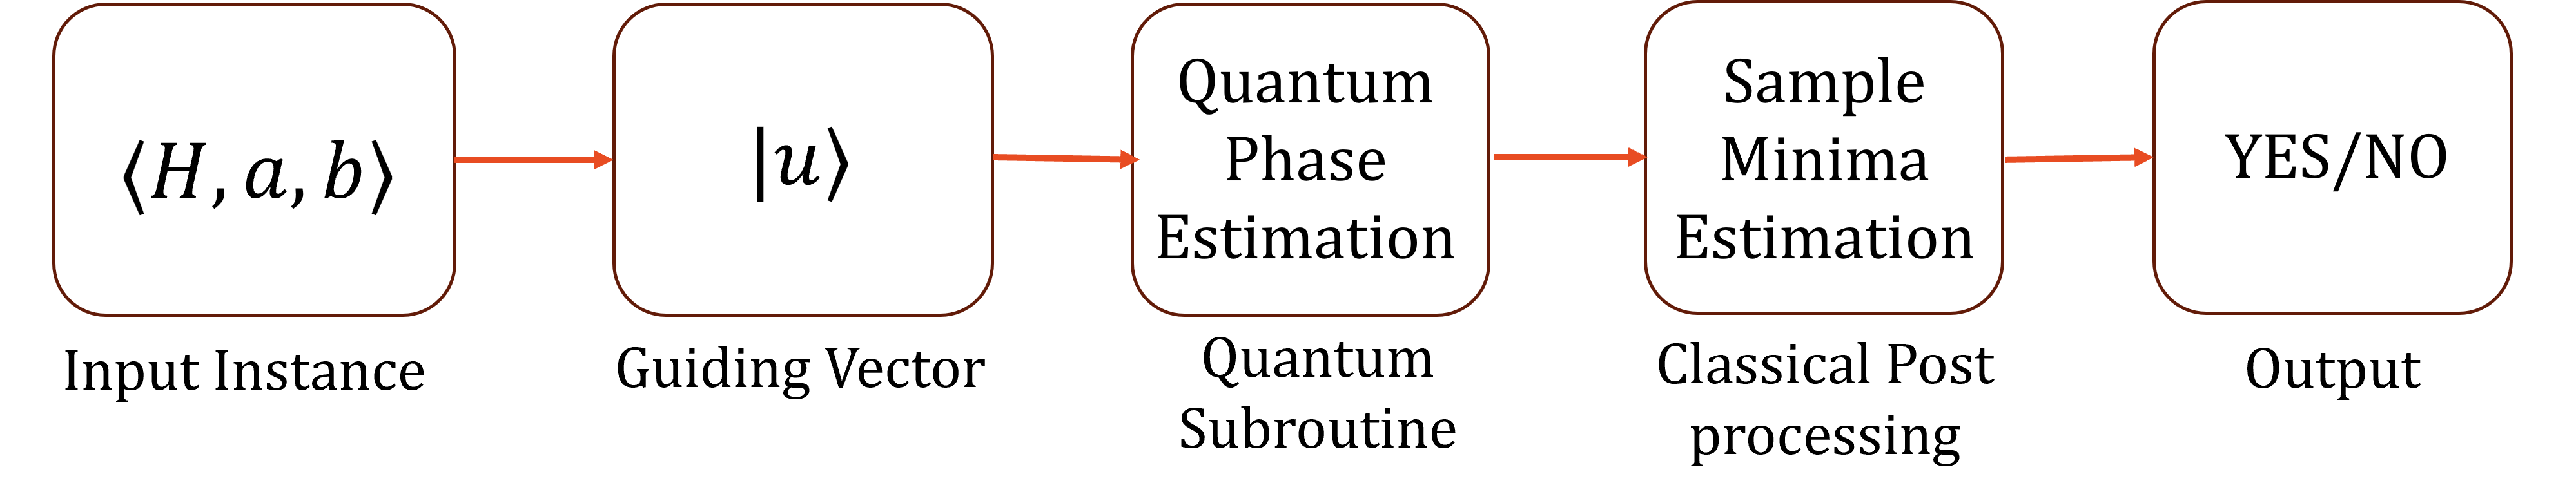
\includegraphics[width=0.90\textwidth]{pics/patent-1.png}
    \caption{The key steps in universal quantum algorithm design.  }
    \label{fig:master-algo}
\end{figure}

\begin{itemize}
    \item $\mathsf{Step\ I}$: A polynomial depth quantum circuit produces a guided state $\ket{\uu}$ using the $\mathsf{GENERATE\ GS}$ algorithm.
    \item $\mathsf{Step\ II}$: The guided state $\ket{\uu}$ is input into the quantum phase estimation algorithm. We utilize a quantum phase estimation algorithm for this purpose.
    \item $\mathsf{Step\ III}$: The algorithm is repeated for $\textrm{poly}\big(\frac{1}{\gamma}\big)$ to collate the sample set $S$. \textbf{Note}: this set contains the minimum eigenvalue as its smallest element (with high success probability).
    \item $\mathsf{Step\ IV}$: Run the $\mathsf{FIND\ MINIMUM\ ELEMENT}$ algorithm on the sample set $S$. Compare the output value with the input parameters $a$ and $b$, and declare the result accordingly.
\end{itemize}
The proof of the algorithm's correctness follows directly from the proof of its correctness given in its steps. The correctness of the quantum phase estimation algorithm is given in Section \ref{sec:comp_prob}. The design and analysis of the  $\mathsf{GENERATE\ GS}$ and  $\mathsf{FIND\ MINIM\ ELEMENT}$  algorithms are given in Subsection \ref{subsec:patent-2}.\newline
In the following three sections, we present the algorithm for $\mathsf{GENERATE\ GS}$ and provide a proof of its optimality (assuming certain complexity-theoretic assumptions).


\subsubsection{Generating the Guiding State: $\mathsf{GENERATE\ GS}$ algorithm }\label{subsec:patent-2}
This subsection contains the design of the algorithm. \newline
\textbf{Input to the algorithm:}
\begin{equation*}
\begin{array}{ll@{}ll}
\text{An efficient description of a $2$-Local Hamiltonian matrix: }  &\displaystyle  \mathsf{H=\sum_{i=1}^{poly(n)}H_i}.
\end{array}
\end{equation*}
\textbf{Steps to the algorithm:}
This is a four-step process to generate a guiding state for the input Hamiltonian $H$.
\begin{itemize}
    \item $\mathsf{Step\ I}$: This step will change the representation of the Hamiltonian operator to the Fourier basis. Technically, it implies expanding the bounded Hermitian operator $\mathsf{H}$ into $\mathsf{Pauli\ Normal\ Form}$. This change of representation is known to be efficient \cite{cubitt2016complexity}.
    \begin{equation}\label{eqn:operator-fourier-trans}
        \mathsf{H=\sum_{s\in \{0,1,2,3\}^n} \hat{f}_s\chi_s}
    \end{equation}
    \item $\mathsf{Step\ II}$: This step will check the locality of the Pauli Hamiltonian as given in the diagram. If it is 1-Local, then it outputs the ground state using \ref{thm:z-ham}. Otherwise, it goes to the next step.
    \item $\mathsf{Step\ III}$: For terms with Pauli degree at most two, check for the threshold $\mathsf{m\leq O(log(n))}$. If it's true, then run the phase estimation on the maximally mixed state  
    \begin{equation}\label{eqn:maximally-mixed-state}
        \mathsf{\rho_{gs}:= \Big( \frac{1}{\sqrt{2^{m}}}\sum_{i\in \{0,1\}^m}\ket{i}\bra{i}\Big)\otimes \ket{u}\bra{u} }
    \end{equation}
    where $\mathsf{\ket{u}}$ is a product state over the remaining qubits that does not appear in $\mathsf{complexity\ generator}$ Pauli terms, that is $\mathsf{\{ZZ\}}$ or $\mathsf{\{XX+YY+ZZ\}}$ Pauli terms. If the threshold $\mathsf{m>O(log(n))}$, the fidelity of the ground state with our estimated ground state $\mathsf{\gamma \leq 1/2^m \leq 1/poly(n)}$ \footnote{The fidelity of $\mathsf{\gamma \geq 1/poly(n)}$ is considered desirable; a good guiding state}. Yet there are cases for which the maximally mixed state would give a polynomial-time algorithm for the cases mentioned in \ref{heuristics}.
\end{itemize}
\textbf{Output of the algorithm:} An estimate of the density matrix corresponding to the ground state of the input Hamiltonian $\mathsf{H}$.
\newline
\textbf{Remark}:  The pair $\mathsf{( H,\ \rho_{gs} )}$ is input to $\mathsf{QPE}$, the algorithm that gives an estimate of the minimum eigenvalue in a time proportional to the fidelity of the estimated ground state to the actual ground state, that is $\gamma$.

%%%%%%%%%%%%%%%%%%%%%%%%%%%%%%%%%%%%%%%%%%%%%%%%%%%%%%%%%%%%%%%%
\subsection{Proof of correctness of the algorithm}\label{sec: correctness}

\subsubsection{Resource analysis for $\mathsf{GENERATE\ GS}$ algorithm}
$\mathsf{Step\ I}$ and $\mathsf{II}$ test the types of the Pauli terms. Thus, the maximum steps are upper bounded by the number of terms in the Hamiltonian, that is $\poly(n)$, because the testing algorithms do a finite number of checks on each $\poly(n)$ Hamiltonian term. This step is purely a classical pre-processing. \par
$\mathsf{Step\ III}$ will requires preparing maximally mixed state. Which can be efficiently simulated by performing quantum phase estimation on half of an input maximally entangled state (for which the reduced density matrix is
maximally mixed) and performing fixed-point amplitude amplification to boost the probability of
success coherently. Thus, the time taken by our method to prepare the ground state is upper bounded by $\mathsf{poly(n)}$.

% In the worst case, we achieve the overall between ground state and our estimated ground state to be $\mathsf{\gamma \geq 1/2^m=1/2^{poly(n)}}$. Thus, overall time scales as $\mathsf{T\leq poly(n,1/\gamma)}$.\newline

\begin{comment}
\subsubsection{$\mathsf{GENERATE\ PAULI\ GS}$ Algorithm}
We use the idea of stabilizer state to formalize an algorithm to generate the ground state of constant degree Pauli operators. The algorithm takes a Pauli string as input and outputs an efficient description of the ground space of the associated Pauli operator. This efficient description can be used to generate the ground state using an efficient quantum circuit. \par
\end{comment}

%%%%%%%%%%%%%%%%%%%%%%%%%%%%%%%%%%%%%%% PATENT03 %%%%%%%%%%%%%%%%%%%%%%%%%%%%%%%%%%%%%%%%%%%%%%%%%%%%%%%%%
%\textcolor{green}{\textbf{Subsection \ref{subsec:patent-3} \& \ref{subsec:circ-depth-uqa} are the subject of Invention/patent 3.}}
\subsubsection{Minimum Energy Estimation: $\QPE$ Algorithm}\label{subsec:patent-3}
This $\QPE$ algorithm is used in the same sense and setting as prescribed in Subsection \ref{subsec:qpe}. The details can be directly borrowed from that section without any loss of generality or any conceptual conflict.
%\subsection{End-to-end resource analysis for the Master algorithm}
%%%%%%%%%%%%%%%%%%%%%%%%%%%%%%%%%%%%%%%%%%%%%%%%%%%%%%%
%%%%%%%%%%%%%%%%%%%%%%%%%%%%%%%%%%%%%%%%%%%%%%%%%%%%%%%
%%%%%%%%%%%%%%%%%%%%%%%%%%%%%%%%%%%%%%%%%%%%%%%%%%%%%%%


%%%%%%%%%%%%%%%%%%%%%%%%%%%%%%%%%%%%%%%   PATENT02   %%%%%%%%%%%%%%%%%%%%%%%%%%%%%%%

%\textcolor{green}{\textbf{Subsection \ref{subsec:patent-2} is the subject of Invention/patent 2.}}

%%%%%%%%%%%%%%%%%%%%%%%%%%%%%%%%%%%%%%%%%%%%%%%%%%%%%%%%%%%%%%%

%%%%%%%%%%%%%%%%%%%%%%%
%%%%%%%%%%%%%%%%%%%%%%%
\section{Robustness of the Hierarchy}\label{sec: oracle-separatoion}
\subsection{Oracle Separation of Levels in the Hierarchy}
Various levels in the $\ms{QMAH}$ hierarchy can be related as follows.
\begin{theorem}
    $\forall i\in \N,\ \ms{QMAH_i}\subseteq  \ms{QMAH_{i+1}}$
\end{theorem}
\textbf{Proof}: This asserts any level in the hierarchy, say $\ms{QMAH_i}$, can be simulated efficiently by $\ms{QMA_{i+1}}$. Notice $\ms{QMAH_i\subseteq BQTIME(2^{O(log^i n)})}$ while, $\ms{QMAH_{i+1}\subseteq BQTIME(2^{O(log^{i+1} n)})}$. Since $\ms{BQTIME(2^{O(log^i n)})\subseteq BQTIME(2^{O(log^{i+1} n)})}$, we have $\ms{QMAH_i\subseteq QMAH_{i+1}}$ as a consequence.\qed

\begin{conj}
    $\forall\ i\in \mathbb{N},\  \ms{QMAH}_i \subsetneq \ms{QMAH}_{i+1}.$
\end{conj}
We conjecture there exists some problem in $\ms{QMAH}_{i+1}$ that is not in $\ms{QMAH}_{i+1}$. Since an unconditional proof for the conjecture would imply $\ms{BQP} \neq \ms{QMA}$, we resort to providing an oracular argument for the conjecture.
\begin{theorem}
    $\forall\ i\in \N$, there exists an oracle $O$ such that $(\ms{QMAH}_i)^O \neq (\ms{QMAH}_{i+1})^O $.
\end{theorem}
\textbf{Proof}: The oracle separation method is inspired by the technique by \cite{Kintala1980-yv} that has been used to separate $\beta_{k+1}\mathsf{P}$ from $\beta_k\mathsf{P}$ using an oracle $\mathsf{O_c}$. The key difference is that we have modified the oracle with Simon's oracle (say $\mathsf{O_q}$) to form a hybrid oracle (say, $\mathsf{O_{qc}}$). Then we argue the hybrid oracle suffices to prove the existence of a problem that is in  $(\ms{QMAH_{i+1}})^{O_{qc}}$ but not in ($\ms{QMAH_{i}})^{O_{qc}}$. \qed
%%%%%%%%%%%%%%%%%%%%%%%%%%%%%%%%%%%%%%%%%%%%%%%%%%%%%%%%%%%%%%%
%%%%%%%%%%%%%%%%%%%%%%%%%%%%%%%%%%%%%%%%%%%%%%%%%%%%%%%%%%%%%%%


%\subsection{ $\ms{QMA}$ contains an infinite number of Time constructible function outside $\ms{BQP}$ }
%(To be updated)
%%%%%%%%%%%%%%%%%%%%%%%%%%%%%%%%%%%%%%%%%%%%%%%%%%%%%%%%%%%%%%%
%%%%%%%%%%%%%%%%%%%%%%%%%%%%%%%%%%%%%%%%%%%%%%%%%%%%%%%%%%%%%%%%%
\section{Discussion, Conclusion and Outlook}
We have proposed two infinite hierarchies in $\mathsf{QMA}$ by quantifying quantum nondeterminism as a tunable computational resource. A variant of $\mathsf{Local\ Hamiltonian}$ has been proven to be a complete natural problem for the classes in the hierarchies. Furthermore, we consider our work to open exciting directions for further research, some of which we will discuss now.\par

First, similar to the hierarchy between $\mathsf{BQP}$ and $\mathsf{QMA}$, one can think of a hierarchy between  $\NP$  and $\mathsf{QMA}$. We suspect that another variant of the $\mathsf{guidable}$ $\LH$$(\gamma, \delta)$ problem could be a potential candidate for complete problems in the hierarchy if the promise gap value $\delta$ is defined as a tunable parameter rather than $\gamma$, the guidance value. This is mainly due to the fact that $k$-$\LH$$(\gamma, \delta)$ with $\delta=O(1)$ is  $\NP$-complete while it is $\mathsf{QMA}$-complete for $\delta=1/\poly(n)$. It would be interesting to look for the implications of this hierarchical characterization on the quantum $\PCP$ conjecture, which asks if promise gap amplification is possible for $\mathsf{QMA}$-complete problems.
\par

%Second, it would be a mathematically elegant exercise to fit a hierarchy between $\QCMA$ and $\mathsf{QMA}$. Recently, Nehoran \& Zhandry \cite{nehoran2023computational} defined a class between them called $\mathsf{cloneable}$-$\mathsf{QMA}$ which fits between them as $\QCMA \subseteq \mathsf{cloneable}$-$\QMA \subseteq \QMA$. The quantifiable resource would be the degree of imperfect cloning of quantum witnesses; the $\QCMA$ witnesses are fully cloneable, while $\mathsf{QMA}$-complete witnesses are poorly cloneable. The proposal of a complete problem for the classes in the hierarchy seems to require fresh thinking.\par

%Second, the completeness of $\mathsf{BQP}$ has been studied via many-to-one deterministic polynomial-time reductions (Karp reductions). This is motivated by the open problem $\P \neq \BQP$. There appears to be virtually no study to understand $\mathsf{BQP}$-completeness in terms of $\BQNC$ reduction. There are two motivations to study this: (i) in the classical case, $\mathsf{P}$-completeness is based on $\NC$ reduction, which is motivated by the problem $\P \neq \NC$, and (ii) $\BQNC$ is conjectured to be strictly smaller than $\mathsf{BQP}$, thus such a reduction can assist in understanding the problem $\BQNC \neq \BQP$. Yet another reason could be that the class $\mathsf{P}$ and $\BQNC$ are considered incomparable\footnote{It is conjectured that (i) $\P \not\subset \BQNC$, and (ii) $\BQNC \not\subset \P$}. Thus, a $\mathsf{P}$-transducer and a $\BQNC$-transducer are likely to possess incomparable reduction capabilities. Thus, redefining $\mathsf{BQP}$-completeness in terms of $\BQNC$ reductions would yield novel insights.\par

%Fourth, we have placed several new problems in the $\BQNC$ hierarchy and conjectured that they are complete under the appropriate notion of reduction. We propose logarithmic space reduction as an appropriate reduction choice, and this also resonates with the study of the problem $\NC \neq \BQNC$. This would be a challenging but interesting exercise to determine the suitable notion of reduction and to prove the completeness of the proposed problems.\par 

Second, our current investigation has fine-grained the complexity of the $\mathsf{Local\ Hamiltonian}$ problem and its variants. The $\mathsf{Local\ Hamiltonian}$ problem is useful in quantum many-body physics; thus, fine-graining might provide insight into those systems.  Recently, a study was conducted to relate the complexity of computing certain types of symmetry in quantum states \cite{rethinasamy2024quantum}. It has been established that computing a certain form of symmetry of a quantum state is $\mathsf{BQP}$-complete. Thus, it would be interesting to fine-tune the complexity of these problems within our hierarchy and then develop a physical interpretation of this classification.\par
We believe that the study we have initiated in this work would provide new physical insights and perspectives on many-body quantum systems under consideration.

%%%%%%%%%%%%%%%%%%%%%%%%%%%%%%%%%%%%%%%%%%%%%%%%%%%%%
%%%%%%%%%%%%%%%%%%%%%%%%%%%%%%%%%%%%%%%%%%%%%%%%%%%%%%%%%%%%%
%%%%%%%%%%%%%%%%%%%%%%%%%%%%%%%%%%%%%%%%%%%%%%%%%%%%%%%%%%
\section{References}
%%%%%%%%%%%%%%%%%%%%%%%%%%%%%%%%%%%%%%%%%%%%%%%%%%%%%%%%%%%%
%\nocite{*}
\bibliographystyle{alpha}
\bibliography{references}
%%%%%%%%%%%%%%%%%%%%%%%%%%%% Appendix -one %%%%%%%%%%%%%%%%%%%%%%%%%
%%%%%%%%%%%%%%%%%%%%%%%%%%%%%%%%%%%%%%%%%%%%%%%%%%%%%%%%%%%%%
%%%%%%%%%%%%%%%%%%%%%%%%%%%%%%%%%%%%%%%%%%%%%%%%%%%%%%%%%%
%\section{Appendix I: Remarks about a quantum Hierarchy in $\ms{QCMA}$}
\newpage
\section{Appendix I: A review of Hamiltonian complexity theory}
We will briefly look at some important results from quantum complexity theory, like the definition of $\mathsf{QMA}$ and $\mathsf{QCMA}$ classes\footnote{They are $\mathsf{promise}$-$\mathsf{QMA}$ and $\mathsf{promise}$-$\mathsf{QCMA}$, respectively. See \cite{gharibian2024guest} to discern them.} and some versions of the $\mathsf{Local\ Hamiltonian}$ problem. A rigorous account of these classes can be found in \cite{gharibian2024guest}. We briefly recap the quantum Merlin-Arthur protocol, as our definitions of hierarchies within $\mathsf{QMA}$ are based on this setup. The notion of \textbf{$\mathsf{P}$-$\mathsf{uniform}$} circuit family will be frequently used to have a rigorous definition of all the quantum complexity classes discussed here.
\begin{definition}
    [$\mathsf{P}$-$\mathsf{uniform}$ quantum circuit family] A family of quantum circuits $\{Q_n\}$ is called $\mathsf{P}$-$\mathsf{uniform}$ if there exists a polynomial-time deterministic Turing machine $M$ which, given as input $1^n$, outputs a classical description of $Q_n$.  
\end{definition}


\subsubsection{Quantum Merlin-Arthur Protocol}\label{subsec:qma-protocol}
A $\mathsf{QMA}$ verification procedure $V$ is $\mathsf{P}$-$\mathsf{uniform}$ quantum circuit family $\{V_x:x\in \{0,1\}^*\}$, together with functions $\mm:\N\rightarrow\N$ and $\kk:\N\rightarrow\N$. The function $\mm$ specifies the length of Merlin's message/witness to Arthur, and it is assumed that each circuit $V_x$ acts on $\mm(|x|)+\kk(|x|)$ qubits. The second function $\kk$ specifies the required ancillary qubits.\newline
\\
$\mathsf{Protocol}$: ($\mm$-qubit $\mathsf{QMA}$ verification procedure) Consider the following process for a string $x\in \{0,1\}^*$ and a quantum state $\ket{\psi}$ on $m$ qubits:
\begin{enumerate}
    \item Run the circuit $V_x$ on the input $\ket{\psi}\ket{0^k}$.
    \item Measure the first qubit of the resulting state on a standard basis, interpreting the outcome $1$ as $\mathsf{accept}$ and outcome $0$ as $\mathsf{reject}$.
\end{enumerate}
The probability associated with two possible outcomes will be denoted accordingly by $\mathsf{Pr}[V_x\ \mathsf{accepts}\ \ket{\psi}]$ and $\mathsf{Pr}[V_x\ \mathsf{reject}\ \ket{\psi}]$. Now, the formal definition for the complexity class $\mathsf{QMA}$ is as follows.

\begin{definition}
    [$\mathsf{QMA}$ complexity class] A promise problem $\mathsf{A=(A_{yes},\ A_{no})}$ is in $\mathsf{QMA}$ if and only if there exists a $\mathsf{P}$-$\mathsf{uniform}$ quantum circuit family $\{V_n\}$ and a polynomial $p(n)$, where $V_n$ takes as input a string $\xx\in \{0,1\}^*$ with $|\xx|=n$, and a $p(n)$-qubit quantum state $\si$ and decides on acceptance or rejection of $\xx$ such that 
    \begin{itemize}
        \item if $\xx\in \mathsf{A_{yes}} \implies$ $\exists\si\in (\C^2)^{\otimes p(n)}$, $\mathsf{Pr[V_n\ accepts\ \ket{\psi}]}$ $\geq 2/3$.
        \item if $\xx\in \mathsf{A_{no}} \implies $ $\forall \si\in (\C^2)^{\otimes p(n)}$, $\mathsf{Pr[V_n\ accepts\ \ket{\psi}]}$ $\leq 1/3$.
    \end{itemize}
\end{definition}
One can easily see that both the witness and verification algorithms require only a polynomial amount of quantum resources with respect to the input size. Merlin can use a $\poly(n)$ number of qubits to encode the witness, while Arthur can use a polynomial-depth quantum circuit for the verification. The complexity class $\QCMA$ deals with the case where Merlin's proof is restricted to be a classical string of $\poly(n)$ size, while Arthur continues to be a $\poly(n)$ depth quantum circuit.

\begin{definition}
    [$\QCMA$ complexity class] A promise problem $\mathsf{A=(A_{yes},\ A_{no})}$ is in   $\QCMA$ if and only if there exists $\mathsf{P}$-$\mathsf{uniform}$ quantum circuit family $\{V_n\}$ and a polynomial $p(n)$, where $V_n$ takes as input a string $\xx\in \{0,1\}^*$ with $|\xx|=n$, and a $p(n)$-bit string $\zz\in \{0,1\}^{p(n)}$ and decides on acceptance or rejection of $\xx$ such that 
    \begin{itemize}
        \item if $\xx\in \mathsf{A_{yes}} \implies$ $\exists \ket{\zz}\in \{0,1\}^{p(n)},$ $\mathsf{Pr[V_n\ accepts\ \ket{\zz}]}$ $\geq 2/3$
        \item if $\xx\in \mathsf{A_{no}} \implies$ $\forall \ket{\zz} \in \{0,1\}^{p(n)},$ $\mathsf{Pr[V_n\ accepts\ \ket{\zz}]}$ $\leq 1/3.$
    \end{itemize}
\end{definition}

It is an open problem if $\mathsf{QMA}$ and $\QCMA$ are indeed distinct classes. The primary difference lies in the nature of the witness. There is some evidence that quantum witnesses should give a richer class \cite{vidick2016quantum}. In a relativized world, they are distinct because of a quantum oracle that separates $\mathsf{QMA}$ from $\QCMA$ \cite{aaronson2007quantum}.

%%%%%%%%%%%%%%%%%%%%%%%%%%%%%%%%%%%%%%%%%%%%%%%%%%%%%%%%%%%%%%%%%%%%%%%%%%%%%%%%%%%%%%%%%%%%%%%%%%%%
\subsubsection{$k$-$\mathsf{Local\ Hamiltonian}$ ($\LH$) Problem}\label{subsec: loc ham variants.}

We will frequently discuss the local Hamiltonian problem and several of its variants throughout the paper. A formal definition of the (promise) problem is as follows. 
\begin{prob}
     [$k$-$\mathsf{Local\ Hamiltonian}$ problem: $k$-$\LH$($\delta$)] The promise problem $k$-Local Hamiltonian is defined as a tuple $\langle H,\ a,\ b\rangle$. \newline
$\Input$: We are given a $k$-local Hamiltonian on $n$ qubits $H=\sum_{j=1}^{r}H_j$ with $r=\poly(n)$. Each Hermitian matrix $H_j\in \HH_k$ has a bounded operator norm $\norm{H_j} \leq 1$, and its entries are specified by $\poly(n)$ bits. In addition, we are given two constants $a$ and $b$ with $|b-a|\geq \delta > 0$.\newline
$\Promise$: For any given instance, either of the two cases below holds. \begin{itemize}
    \item For YES instances, $\lambda_0(H)\leq a$.
    \item For NO instances, $\lambda_0(H)\geq b$.
\end{itemize}
$\Output$: Decide which is the case.
\label{def:k-LH}
\end{prob}
This problem has been shown to be complete in the class $\mathsf{QMA}$ when the parameters $k$ and $\delta$ lie within a certain range.
\begin{theorem}
[\cite{kempe2004complexity}] 2-$\mathsf{LH(\delta)}$ problem with the promise gap $\delta \geq \big(\frac{1}{\poly(n)}\big)$ is $\mathsf{QMA}$-complete under Karp reduction.
\end{theorem}
$k$-$\LH$ problem is a quantum generalization of Constraint Satisfaction Problems; the classical problem is the special case where each matrix $H_j$ is diagonal in the computational basis and only contains 0's and 1's. The $k$-$\LH$ problem has several variants with varying difficulty levels. Now, we will see some of its important variants. Later, we will design a couple of new variants of $k$-$\LH$ to incorporate them into our hierarchies in $\mathsf{QMA}$.
%%%%%%%%%%%%%%%%%%%%%%%%%%%%%%%%%%%%%%%%%%%%%%%%%%%%%%%%%%%%%%%%%%%%%%%%%%%%%%%%%%%%%%%%%%%



\begin{comment}
\textbf{Remark:} From a complexity-theoretic point of view, the class $\mathsf{QMA}$ is robust even if the underlying field of the complex vector space is restricted to the real field.

\begin{prob}
    [$k$-Local REAL Hamiltonian]: In this case, the Hamiltonian (matrices) in the definition \ref{def:k-LH} can only belong to the real part of the vector space, that is, $H_{j} \in \mathbb{R}^{N\times N}$.
\end{prob}

\begin{theorem}
    [\cite{BL08}] $k$-Local REAL Hamiltonian with the promise gap $\delta\geq\frac{1}{\poly(n)}$ is $\mathsf{QMA}$-complete under Karp reduction.
    \label{thm:bl08}
\end{theorem}

Thus, without any loss of generality, we assume that all the subsequent problems have local Hamiltonians defined exclusively over the real part of the underlying vector space. %\textbf{Note}: Every Hilbert space is a special type of complex vector space.

    \textbf{Lemma-1:}[BL08] At most two of the Pauli matrices (tensored with identities) are sufficient to (efficiently) represent any individual $k$-local Hermitian term ($H_{ij}$ matrices). Or, 
$$H_{ij}= I\otimes...\otimes\sigma_i^l\otimes...\otimes\sigma_j^l\otimes...\otimes I$$   where $l \in\{1,\ 3\}$.\\
\end{comment}


\subsubsection{Some Variants of $k$-$\LH$ Problem}\label{subsubsec:variantsLH}
%%%%%%%%%%%%%%%%%%%%%%%%%%%%%%%%%%%%%%%%%%%%%%%%%%%%%%%%%%%%%%%%%%%%%%%%%%%%%%%%%%%%%%%%%%%%%%%%%%%%


\textbf{Variant I: $\mathsf{Guided}$ $k$-$\mathsf{Local\ Hamiltonian}$ problem: $\GLH$$\mathsf{(k,\gamma,\delta)}$.} Like $\mathsf{QMA}$, there are several complete problems for $\QCMA$. We especially mention a particular $\QCMA$-complete problem named the Guidable local Hamiltonian problem ($\GaLH$). To fully appreciate this problem, we need to consider a precursor problem, the Guided Local Hamiltonian ($\GLH$) problem, which is $\mathsf{BQP}$-complete. This was introduced by Gharibian \& Le Gall \cite{gharibian2022dequantizing}. They formalized the complexity of $k$-$\LH(\gamma,\delta)$ with a $\mathsf{good}$ guiding state. We give a brief exposition of the $\GLH$ problem.\par
The definition of $\GLH$ consists of three important terminologies as follows:\newline
$\mathsf{Subset\ State}$ (\cite{grilo2015qma}): For any subset $S\subseteq [2^n]_1$, we define the subset state $\ket{S}\in \mathbb{R}^{2^n}$, as the uniform superposition over the elements of $S$. More precisely,
\begin{equation}
    \ket{S}:= \frac{1}{\sqrt{|S|}}\sum_{i\in S}\ket{i}.
\end{equation}
$\mathsf{Guided\ State}$: For a given $k$-$\mathsf{LH}$ problem with Hamiltonian $H$, the unit norm vector $\ket{\uu}\in \mathbb{R}^{2^n}$ is defined to be a guided state if it is a subset state 
$$\ket{\uu}:= \frac{1}{\sqrt{|S|}}\sum_{i\in S}\ket{i}$$ with a non-empty subset $S\subseteq [2^n]_1$ and $|S|=O(\poly(n))$. The last restriction on the size of the subset $S$ is crucial to discern a subset state from a guided state. \newline
$\mathsf{Guidance\ Value}$: For a given $k$-$\LH$ problem with the Hamiltonian $H$, the scalar $\gamma(n)\in [0,\ 1]$ is called the guidance value of the guided state $\ket{\uu}$ $$\gamma(n):=\norm{\Pi_{\mathsf{gs}}\ket{\uu}}^2$$ where $\Pi_{\mathsf{gs}}$ is the projection on the subspace spanned by the ground state of $H$. This quantifies the quality of a guided state. Having these three terminologies at hand, the problem is defined as follows.

\begin{prob}
[\cite{gharibian2022dequantizing}: $\GLH$$\mathsf{(k,\gamma,\delta)}$ problem] The problem is a tuple $\langle H; \ket{\uu};(a,b) \rangle$ with the following characteristics. \newline
$\Input$: (i) a $k$-local Hamiltonian matrix  $H=\sum_{j=1}^{m}H_j$ for an $n$-qubit system such that $\norm{H}\leq 1$, (ii) an efficient description of a semi-classical state $\uu\in \C^{2^n}$ and (iii) promise gap parameter $a,\ b\in \R$ such that $|b-a|\geq \delta>0$. \newline
$\Promise$:
\begin{itemize}
    \item Fidelity with the ground space $\norm{\Pi_{\mathsf{gs}} \ket{\uu}}\geq \gamma$.
    \item Either case (i) $\lambda_0\leq a$ or (ii) $\lambda_0\geq b$ holds.
\end{itemize}
$\Output$:\newline
1. If $\lambda_0(H) \leq a$, output YES. \newline
2. If $\lambda_0(H) \geq b$, output NO.
\end{prob}
Within a certain parameter range, this problem is known to be $\mathsf{BQP}$-complete. Currently, the best-known result is summarized in the following theorem.
\begin{theorem}
    [\cite{cade2022complexity}]: For any $\gamma(n)\in \big(0, 1-\Omega(1/\poly(n))\big)$, constant $k\geq 2$, there exists a promise gap parameter $a,\ b \in [-1,1]$ with $b-a\in \Omega(1/\mathsf{poly}(n))$ such that $\GLH$$\mathsf{(k,\gamma,\delta)}$ is $\mathsf{BQP}$-complete.
\end{theorem}

%%%%%%%%%%%%%%%%%%%%%%%%%%% Problem 2 %%%%%%%%%%%%%%%%%%%%%%%%%%%
\textbf{Variant III: $\mathsf{Guidable}$ $k$-$\mathsf{Local\ Hamiltonian}$ problem: $\GaLH$$\mathsf{(k,\gamma,\delta)}$. }
The idea of Guidable Local Hamiltonian ($\GaLH$) was introduced by Weggemans et al. \cite{weggemans2023guidable}. The key difference between $\GLH$ and $\GaLH$ is that $\GLH$ has the guiding state given as part of the problem. But in $\GaLH$, there is a mere promise of the existence of such a guiding state.
\begin{prob}
    [$\mathsf{Guidable}$ $k$-$\mathsf{Local\ Hamiltonian}$ ($\GaLH$) problem] The problem is a tuple $\langle H;(a,b) \rangle$ with the following characteristics. \newline
    $\Input$: The inputs given are (i) $k$-local Hamiltonian $H=\sum_{j=1}^{m}H_j$ acting on $n$ qubits such that $\norm{H}\leq 1$, (ii) a fidelity parameter $\gamma(p)\in (0,\ 1]$, and (iii) a promise gap parameter $a,\ b\in \R$ such that $|b-a|\geq \delta>0$. \newline
    $\Promise$: We have that either $\lambda_0(H) \leq a$ or $\lambda_0(H) \geq b$ holds, where $\lambda_0(H)$ denotes the ground state energy of $H$.\newline
    $\mathsf{Extra\ promise:}$ Denote $\Pi_{gs}$ for the projection on the subspace spanned by the ground state of $H$. Then, there exists a unitary $V$ implemented by a quantum circuit composed of at most $T=O(\poly(n))$ gates from a set of fixed gates $\mathcal{G}$ that produces the state $\ket{\phi}=V\ket{0}$, which has $\norm{\Pi_{gs}\uu}\geq \gamma$.\newline
    $\Output$:\newline
    1. If $\lambda_0(H) \leq a$, output $\mathsf{YES}$.\newline
    2. If $\lambda_0(H) \geq b$, output $\mathsf{NO}$.
\end{prob}
\begin{theorem}
    [\cite{weggemans2023guidable}] For all $p\in \N$, $k\geq 2$, $\gamma \in \big(\frac{1}{\poly(n)},1-\frac{1}{\poly(n)}\big)$, and $\delta=\Omega \big(1/\poly(n)\big)$, the $\mathsf{GaLH(k,\gamma,\delta)}$ problem is a complete problem for $\QCMA$ under randomized reduction.
\end{theorem}
This result has some very significant implications. Since $\mathsf{P}$, $\mathsf{BQP}$, and $\NP$ are contained in the $\QCMA$, an efficient description of the guiding state must exist if the problem of these classes is reduced to a local Hamiltonian problem. Thus, the bottleneck to solving these problems reduces to finding a guiding state\footnote{This means the complexity of solving the problems in $\QCMA$ can be squeezed to finding a $\mathsf{'good'}$ guiding state for the reduced Local Hamiltonian problem.}. Once we have the guiding state, there is an efficient quantum algorithm to compute the minimum eigenvalue of the problem. See Section \ref{sec:uqa} for further analysis.\par
%The key motivation for mentioning this variant of $k$-$\LH$ is to analyze the problem's defining property, which is difficult to intermediate between $\GLH$ and $k$-$\LH$. As we shall see later, we have defined a variant inspired by the $\GaLH$ problem and placed it in our hierarchy between $\mathsf{BQP}$ and $\QCMA$-$\mathsf{complete}$.


%%%%%%%%%%%%%%%%%%%%%%%%%%%%%%%%%%%%%%%%%%%%%%%%%%%%%%%%%%%%
%%%%%%%%%%%%%%%%%%%%%%%%%%%%%%%%%%%%%%%%%%%%%%%%%%%%%%%%%%%%


\section{Appendix II: A review of an infinite hierarchy between $\ms{P}$ and $\ms{NP}$}
Ladner proposed a hierarchy between $\mathsf{P}$ and $\NP$ assuming $\P \neq \NP$ \cite{ladner1975structure} is true. But the problems in the hierarchy were mathematically contrived. Kintala \& Fischer \cite{Kintala1980-yv} defined another hierarchy using the concept of a Turing machine with access to a limited amount of classical nondeterminism. Later, the hierarchy was populated with several natural problems, such as a specific variant of $\SAT$, $\mathsf{HAM}$-$\mathsf{CYCLE}$, and $\mathsf{VERTEX}$-$\mathsf{COVER}$ \cite{farr1994problems}.\par
\subsubsection{Classical $\beta$-Hierarchy}\label{sec:classsical-hierarchy}
Informally, $\beta$-$P$ hierarchy is defined as classes of sets accepted by a polynomial-time bounded Turing machine that makes a poly-logarithmic number of non-deterministic steps. By varying the degree of the poly-logarithmic function, we get an infinite hierarchy between $\mathsf{P}$ and $\NP$-complete sets. The next two definitions formalize this notion.
\begin{definition}
    [$\beta$-Hierarchies \cite{Kintala1980-yv}] Let $\mathcal{F}$ be a class of functions, and $\mathcal{C}=\bigcup_{f\in \mathcal{F}} \mathsf{DTIME(f)}$ be the class of sets accepted by deterministic $\mathcal{F}$-time bounded Turing machines. For the total function $\mathsf{g}:\mathbb{N}\rightarrow \mathbb{N}$, $\mathsf{g(n)}$-$\mathcal{C}$ denotes the class of sets accepted by nondeterministic $\mathcal{F}$-time bounded Turing machines making at most $\mathsf{g(n)}$ nondeterministic steps on every input of length $n$.
\end{definition}

\begin{definition}
    [$\beta$-$\mathsf{P}$ Hierarchy \cite{Kintala1980-yv}] For every $k\in \mathbb{N}$, by definition the complexity class $\beta_k\P$=$\bigcup_{c\in \mathbb{N}} \mathsf{(c\cdot log^{k}n)}$-$\mathsf{P}$. Then $\beta$$\mathsf{P}$-hierarchy is $\beta \P= \bigcup_{k\in \N} \beta_k \P$.
\end{definition}
As a consequence of the above definition, the complexity class $\mathsf{P}$ can be thought of as a class of problems that a polynomial-time Turing machine can solve with $O(\log n)$ nondeterministic steps.
\begin{theorem}
    [\cite{Kintala1980-yv}:] With respect to Kintala's $\beta \P$ hierarchy, $\P=\beta_1\P$. 
\end{theorem}
$\Proof$: The proof follows from the fact that the Turing machine can brute force through the space of ${O(\log} n)$ non-deterministic guesses. \textbf{Note}: there are at most $2^{\mathsf{O(log\ n)}}\leq \poly(n)$ possibilities to be explored by the Turing machine.\qed

Subsequent studies have identified several natural problems at various levels of the hierarchy. For example, G. Farr proposed a particular variant of the $\SAT$ problem and proved it to be complete for the various levels. 
\begin{prob}
    [$\beta_k$-$\SAT$ \cite{farr1994problems}] It is defined as the set of all pairs $\langle \phi, V\rangle$ of the formula $\phi$ and the set $V$ of at most $\log^k|\phi|$ variables in $\phi$, for which there exists an assignment $\mathcal{A}$ to all variables in $V$ that forces a satisfying assignment for $\phi$. Note that $\beta_1$-$\SAT$ is $p$-isomorphic to the $\mathsf{P}$-complete complement of the unit resolution problem.
\end{prob}
\begin{theorem}
    [\cite{farr1994problems}] For every $k\in \N$, $\beta_k$-$\SAT$ is a complete problem for $\beta_k$-$\mathsf{P}$ under polynomial-time many-one reduction.
\end{theorem}

%One of the goals of this paper is to explore a similar hierarchy between $\mathsf{BQP}$ and $\mathsf{QMA}$-$\mathsf{complete}$. Then, we propose several natural problems that are complete for the various levels of the quantum hierarchy. Since the $\mathsf{Local\ Hamiltonian}$ ($\LH$) problem is a possible quantum generalization of $\SAT$, we review $\LH$ and some of its variants. In the later section, we design new variants of the $\LH$ problem that serve as a complete problem for a given level of the quantum hierarchy. \newline

\end{document}

